% Options for packages loaded elsewhere
\PassOptionsToPackage{unicode}{hyperref}
\PassOptionsToPackage{hyphens}{url}
\documentclass[
]{book}
\usepackage{xcolor}
\usepackage{amsmath,amssymb}
\setcounter{secnumdepth}{5}
\usepackage{iftex}
\ifPDFTeX
  \usepackage[T1]{fontenc}
  \usepackage[utf8]{inputenc}
  \usepackage{textcomp} % provide euro and other symbols
\else % if luatex or xetex
  \usepackage{unicode-math} % this also loads fontspec
  \defaultfontfeatures{Scale=MatchLowercase}
  \defaultfontfeatures[\rmfamily]{Ligatures=TeX,Scale=1}
\fi
\usepackage{lmodern}
\ifPDFTeX\else
  % xetex/luatex font selection
\fi
% Use upquote if available, for straight quotes in verbatim environments
\IfFileExists{upquote.sty}{\usepackage{upquote}}{}
\IfFileExists{microtype.sty}{% use microtype if available
  \usepackage[]{microtype}
  \UseMicrotypeSet[protrusion]{basicmath} % disable protrusion for tt fonts
}{}
\makeatletter
\@ifundefined{KOMAClassName}{% if non-KOMA class
  \IfFileExists{parskip.sty}{%
    \usepackage{parskip}
  }{% else
    \setlength{\parindent}{0pt}
    \setlength{\parskip}{6pt plus 2pt minus 1pt}}
}{% if KOMA class
  \KOMAoptions{parskip=half}}
\makeatother
\usepackage{color}
\usepackage{fancyvrb}
\newcommand{\VerbBar}{|}
\newcommand{\VERB}{\Verb[commandchars=\\\{\}]}
\DefineVerbatimEnvironment{Highlighting}{Verbatim}{commandchars=\\\{\}}
% Add ',fontsize=\small' for more characters per line
\usepackage{framed}
\definecolor{shadecolor}{RGB}{248,248,248}
\newenvironment{Shaded}{\begin{snugshade}}{\end{snugshade}}
\newcommand{\AlertTok}[1]{\textcolor[rgb]{0.94,0.16,0.16}{#1}}
\newcommand{\AnnotationTok}[1]{\textcolor[rgb]{0.56,0.35,0.01}{\textbf{\textit{#1}}}}
\newcommand{\AttributeTok}[1]{\textcolor[rgb]{0.13,0.29,0.53}{#1}}
\newcommand{\BaseNTok}[1]{\textcolor[rgb]{0.00,0.00,0.81}{#1}}
\newcommand{\BuiltInTok}[1]{#1}
\newcommand{\CharTok}[1]{\textcolor[rgb]{0.31,0.60,0.02}{#1}}
\newcommand{\CommentTok}[1]{\textcolor[rgb]{0.56,0.35,0.01}{\textit{#1}}}
\newcommand{\CommentVarTok}[1]{\textcolor[rgb]{0.56,0.35,0.01}{\textbf{\textit{#1}}}}
\newcommand{\ConstantTok}[1]{\textcolor[rgb]{0.56,0.35,0.01}{#1}}
\newcommand{\ControlFlowTok}[1]{\textcolor[rgb]{0.13,0.29,0.53}{\textbf{#1}}}
\newcommand{\DataTypeTok}[1]{\textcolor[rgb]{0.13,0.29,0.53}{#1}}
\newcommand{\DecValTok}[1]{\textcolor[rgb]{0.00,0.00,0.81}{#1}}
\newcommand{\DocumentationTok}[1]{\textcolor[rgb]{0.56,0.35,0.01}{\textbf{\textit{#1}}}}
\newcommand{\ErrorTok}[1]{\textcolor[rgb]{0.64,0.00,0.00}{\textbf{#1}}}
\newcommand{\ExtensionTok}[1]{#1}
\newcommand{\FloatTok}[1]{\textcolor[rgb]{0.00,0.00,0.81}{#1}}
\newcommand{\FunctionTok}[1]{\textcolor[rgb]{0.13,0.29,0.53}{\textbf{#1}}}
\newcommand{\ImportTok}[1]{#1}
\newcommand{\InformationTok}[1]{\textcolor[rgb]{0.56,0.35,0.01}{\textbf{\textit{#1}}}}
\newcommand{\KeywordTok}[1]{\textcolor[rgb]{0.13,0.29,0.53}{\textbf{#1}}}
\newcommand{\NormalTok}[1]{#1}
\newcommand{\OperatorTok}[1]{\textcolor[rgb]{0.81,0.36,0.00}{\textbf{#1}}}
\newcommand{\OtherTok}[1]{\textcolor[rgb]{0.56,0.35,0.01}{#1}}
\newcommand{\PreprocessorTok}[1]{\textcolor[rgb]{0.56,0.35,0.01}{\textit{#1}}}
\newcommand{\RegionMarkerTok}[1]{#1}
\newcommand{\SpecialCharTok}[1]{\textcolor[rgb]{0.81,0.36,0.00}{\textbf{#1}}}
\newcommand{\SpecialStringTok}[1]{\textcolor[rgb]{0.31,0.60,0.02}{#1}}
\newcommand{\StringTok}[1]{\textcolor[rgb]{0.31,0.60,0.02}{#1}}
\newcommand{\VariableTok}[1]{\textcolor[rgb]{0.00,0.00,0.00}{#1}}
\newcommand{\VerbatimStringTok}[1]{\textcolor[rgb]{0.31,0.60,0.02}{#1}}
\newcommand{\WarningTok}[1]{\textcolor[rgb]{0.56,0.35,0.01}{\textbf{\textit{#1}}}}
\usepackage{longtable,booktabs,array}
\usepackage{calc} % for calculating minipage widths
% Correct order of tables after \paragraph or \subparagraph
\usepackage{etoolbox}
\makeatletter
\patchcmd\longtable{\par}{\if@noskipsec\mbox{}\fi\par}{}{}
\makeatother
% Allow footnotes in longtable head/foot
\IfFileExists{footnotehyper.sty}{\usepackage{footnotehyper}}{\usepackage{footnote}}
\makesavenoteenv{longtable}
\usepackage{graphicx}
\makeatletter
\newsavebox\pandoc@box
\newcommand*\pandocbounded[1]{% scales image to fit in text height/width
  \sbox\pandoc@box{#1}%
  \Gscale@div\@tempa{\textheight}{\dimexpr\ht\pandoc@box+\dp\pandoc@box\relax}%
  \Gscale@div\@tempb{\linewidth}{\wd\pandoc@box}%
  \ifdim\@tempb\p@<\@tempa\p@\let\@tempa\@tempb\fi% select the smaller of both
  \ifdim\@tempa\p@<\p@\scalebox{\@tempa}{\usebox\pandoc@box}%
  \else\usebox{\pandoc@box}%
  \fi%
}
% Set default figure placement to htbp
\def\fps@figure{htbp}
\makeatother
\setlength{\emergencystretch}{3em} % prevent overfull lines
\providecommand{\tightlist}{%
  \setlength{\itemsep}{0pt}\setlength{\parskip}{0pt}}
\usepackage[]{natbib}
\bibliographystyle{plainnat}
\usepackage{booktabs}
\usepackage{bookmark}
\IfFileExists{xurl.sty}{\usepackage{xurl}}{} % add URL line breaks if available
\urlstyle{same}
\hypersetup{
  pdftitle={Descriptive Statistics for One Variable},
  pdfauthor={Samuel Rowe adapted from Acock (2023)},
  hidelinks,
  pdfcreator={LaTeX via pandoc}}

\title{Descriptive Statistics for One Variable}
\author{Samuel Rowe adapted from Acock (2023)}
\date{2026-08-22}

\begin{document}
\maketitle

{
\setcounter{tocdepth}{1}
\tableofcontents
}
\begin{Shaded}
\begin{Highlighting}[]
\NormalTok{bookdown}\SpecialCharTok{::}\FunctionTok{render\_book}\NormalTok{()}
\end{Highlighting}
\end{Shaded}

\chapter*{Overview}\label{overview}
\addcontentsline{toc}{chapter}{Overview}

Topics:

\begin{enumerate}
\def\labelenumi{\arabic{enumi}.}
\tightlist
\item
  Descriptive Statistics for One Variable
\item
  Exercises
\end{enumerate}

\chapter{Descriptive Statistics fo One Variable}\label{descriptive-statistics-fo-one-variable}

Understanding the central tendency and the distribution of a variable is an essential part of an empirical study. We will utilize Stata to calculate and display descriptive statistics of central tendency, variability, and distribution.

\section{Central Tendency}\label{central-tendency}

For central tendency, we can calculate the mean, median, and mode as previous discussed in SfBE. For measuring central tendency, the choice depends upon the type of variable you are working with. What is the level of measurement? What is the distribution? What are you trying to show?

\begin{tabular}{l|l|l|l}
\hline
Level.of.Measurement & Mode & Median & Mean\\
\hline
Categorical with no order (Nominal), Categorical with Order (Ordinal), Quantitative (Discrete, Continuous, Interval & Yes & No & No\\
\hline
Categorical with no order (Nominal), Categorical with Order (Ordinal), Quantitative (Discrete, Continuous, Interval & Yes & Yes & Yes\\
\hline
Categorical with no order (Nominal), Categorical with Order (Ordinal), Quantitative (Discrete, Continuous, Interval & Yes & Yes & Yes\\
\hline
\end{tabular}

\begin{itemize}
\tightlist
\item
  For nominal categories variables, you can use the mode.
\item
  For ordinal categorical variables, you can use the mode and possibly the mean.
\item
  For quantitative variables, you can use mean, median, and mode.
\end{itemize}

Let's look at an example from the General Social Survey from Acock (2023). We will look at a ordinal categorical variable called ``childs'' which is the number of children in a household.

\begin{Shaded}
\begin{Highlighting}[]
\KeywordTok{use}\NormalTok{ descriptive\_gss, }\KeywordTok{clear}
\KeywordTok{graph} \BaseNTok{bar}\NormalTok{ (}\FunctionTok{count}\NormalTok{) }\KeywordTok{if}\NormalTok{ childs \textgreater{} 0, }\BaseNTok{over}\NormalTok{(childs,gap(0)) }\CommentTok{///}
  \BaseNTok{bar}\NormalTok{(1, lcolor(}\BaseNTok{black}\NormalTok{)) }\BaseNTok{title}\NormalTok{(}\StringTok{"Number of children in families with at least one child"}\NormalTok{) }\CommentTok{///}
  \BaseNTok{caption}\NormalTok{(}\StringTok{"descriptive\_gss.dta"}\NormalTok{) }\BaseNTok{ytitle}\NormalTok{(}\StringTok{"Frequency"}\NormalTok{) lintensity(100)  }
\end{Highlighting}
\end{Shaded}

\begin{figure}
\centering
\pandocbounded{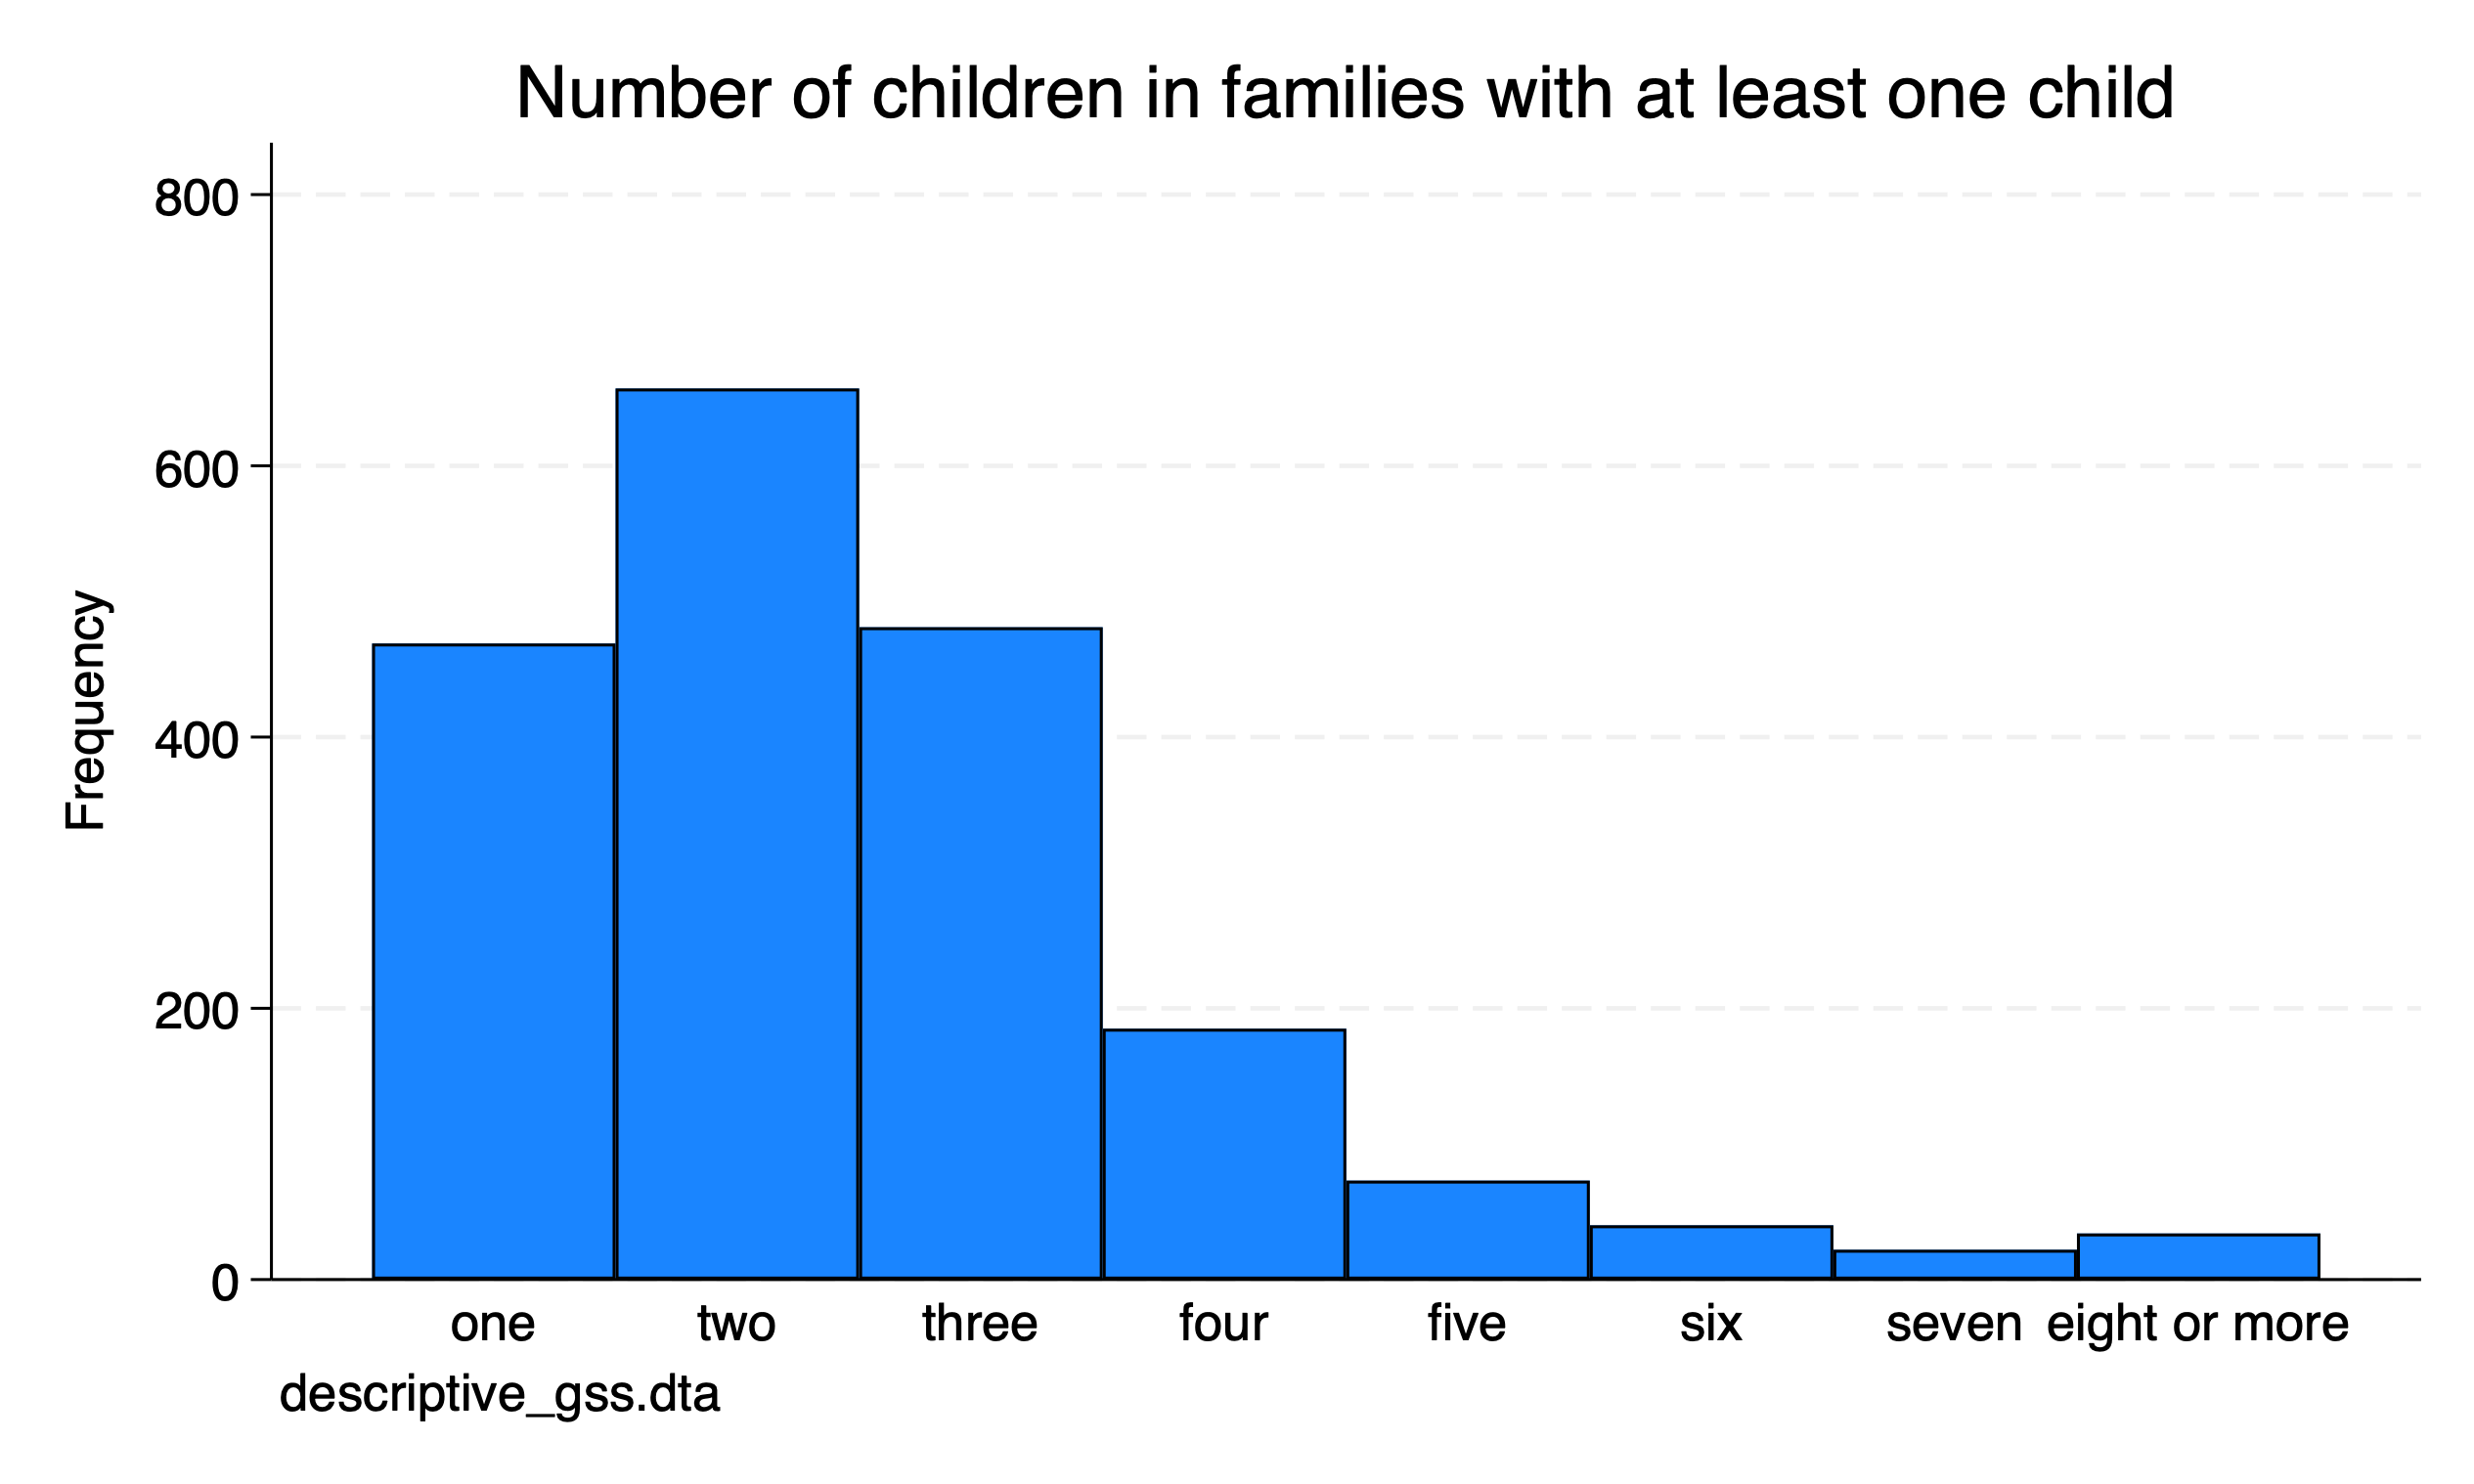
\includegraphics[keepaspectratio,alt={How many children do familes have?}]{week3_graph1.png}}
\caption{How many children do familes have?}
\end{figure}

It is clear that the mode is 2, but what about the median or mean for the ordinal variable?

\begin{Shaded}
\begin{Highlighting}[]
\KeywordTok{summarize}\NormalTok{ childs, details}
\end{Highlighting}
\end{Shaded}

\begin{verbatim}
                     number of children
-------------------------------------------------------------
      Percentiles      Smallest
 1%            1              1
 5%            1              1
10%            1              1       Obs               1,961
25%            2              1       Sum of wgt.       1,961

50%            2                      Mean            2.54819
                        Largest       Std. dev.      1.458909
75%            3              8
90%            4              8       Variance       2.128416
95%            5              8       Skewness       1.468189
99%            8              8       Kurtosis       5.700491
\end{verbatim}

From our summary statistics we can see that family with kids the median is 2 and the mean rounded up to 3. The data are slighly skewed since the mean \textgreater{} median and mean \textgreater{} mode.

\section{Distribution}\label{distribution}

For quantitative data, we want to the dispersion along with central tendency. Are the values concentrated in the middle or are they widely spread out? If we look at hypothetical SAT scores from applications to two universities. Both university have the same mean of 1,000 but different standard deviations are different. One university application SAT scores has a \(SD=100\) and the other university application SAT scores has a \(SD=200\). Let's plot the distribution of these SAT scores.

\begin{figure}
\centering
\pandocbounded{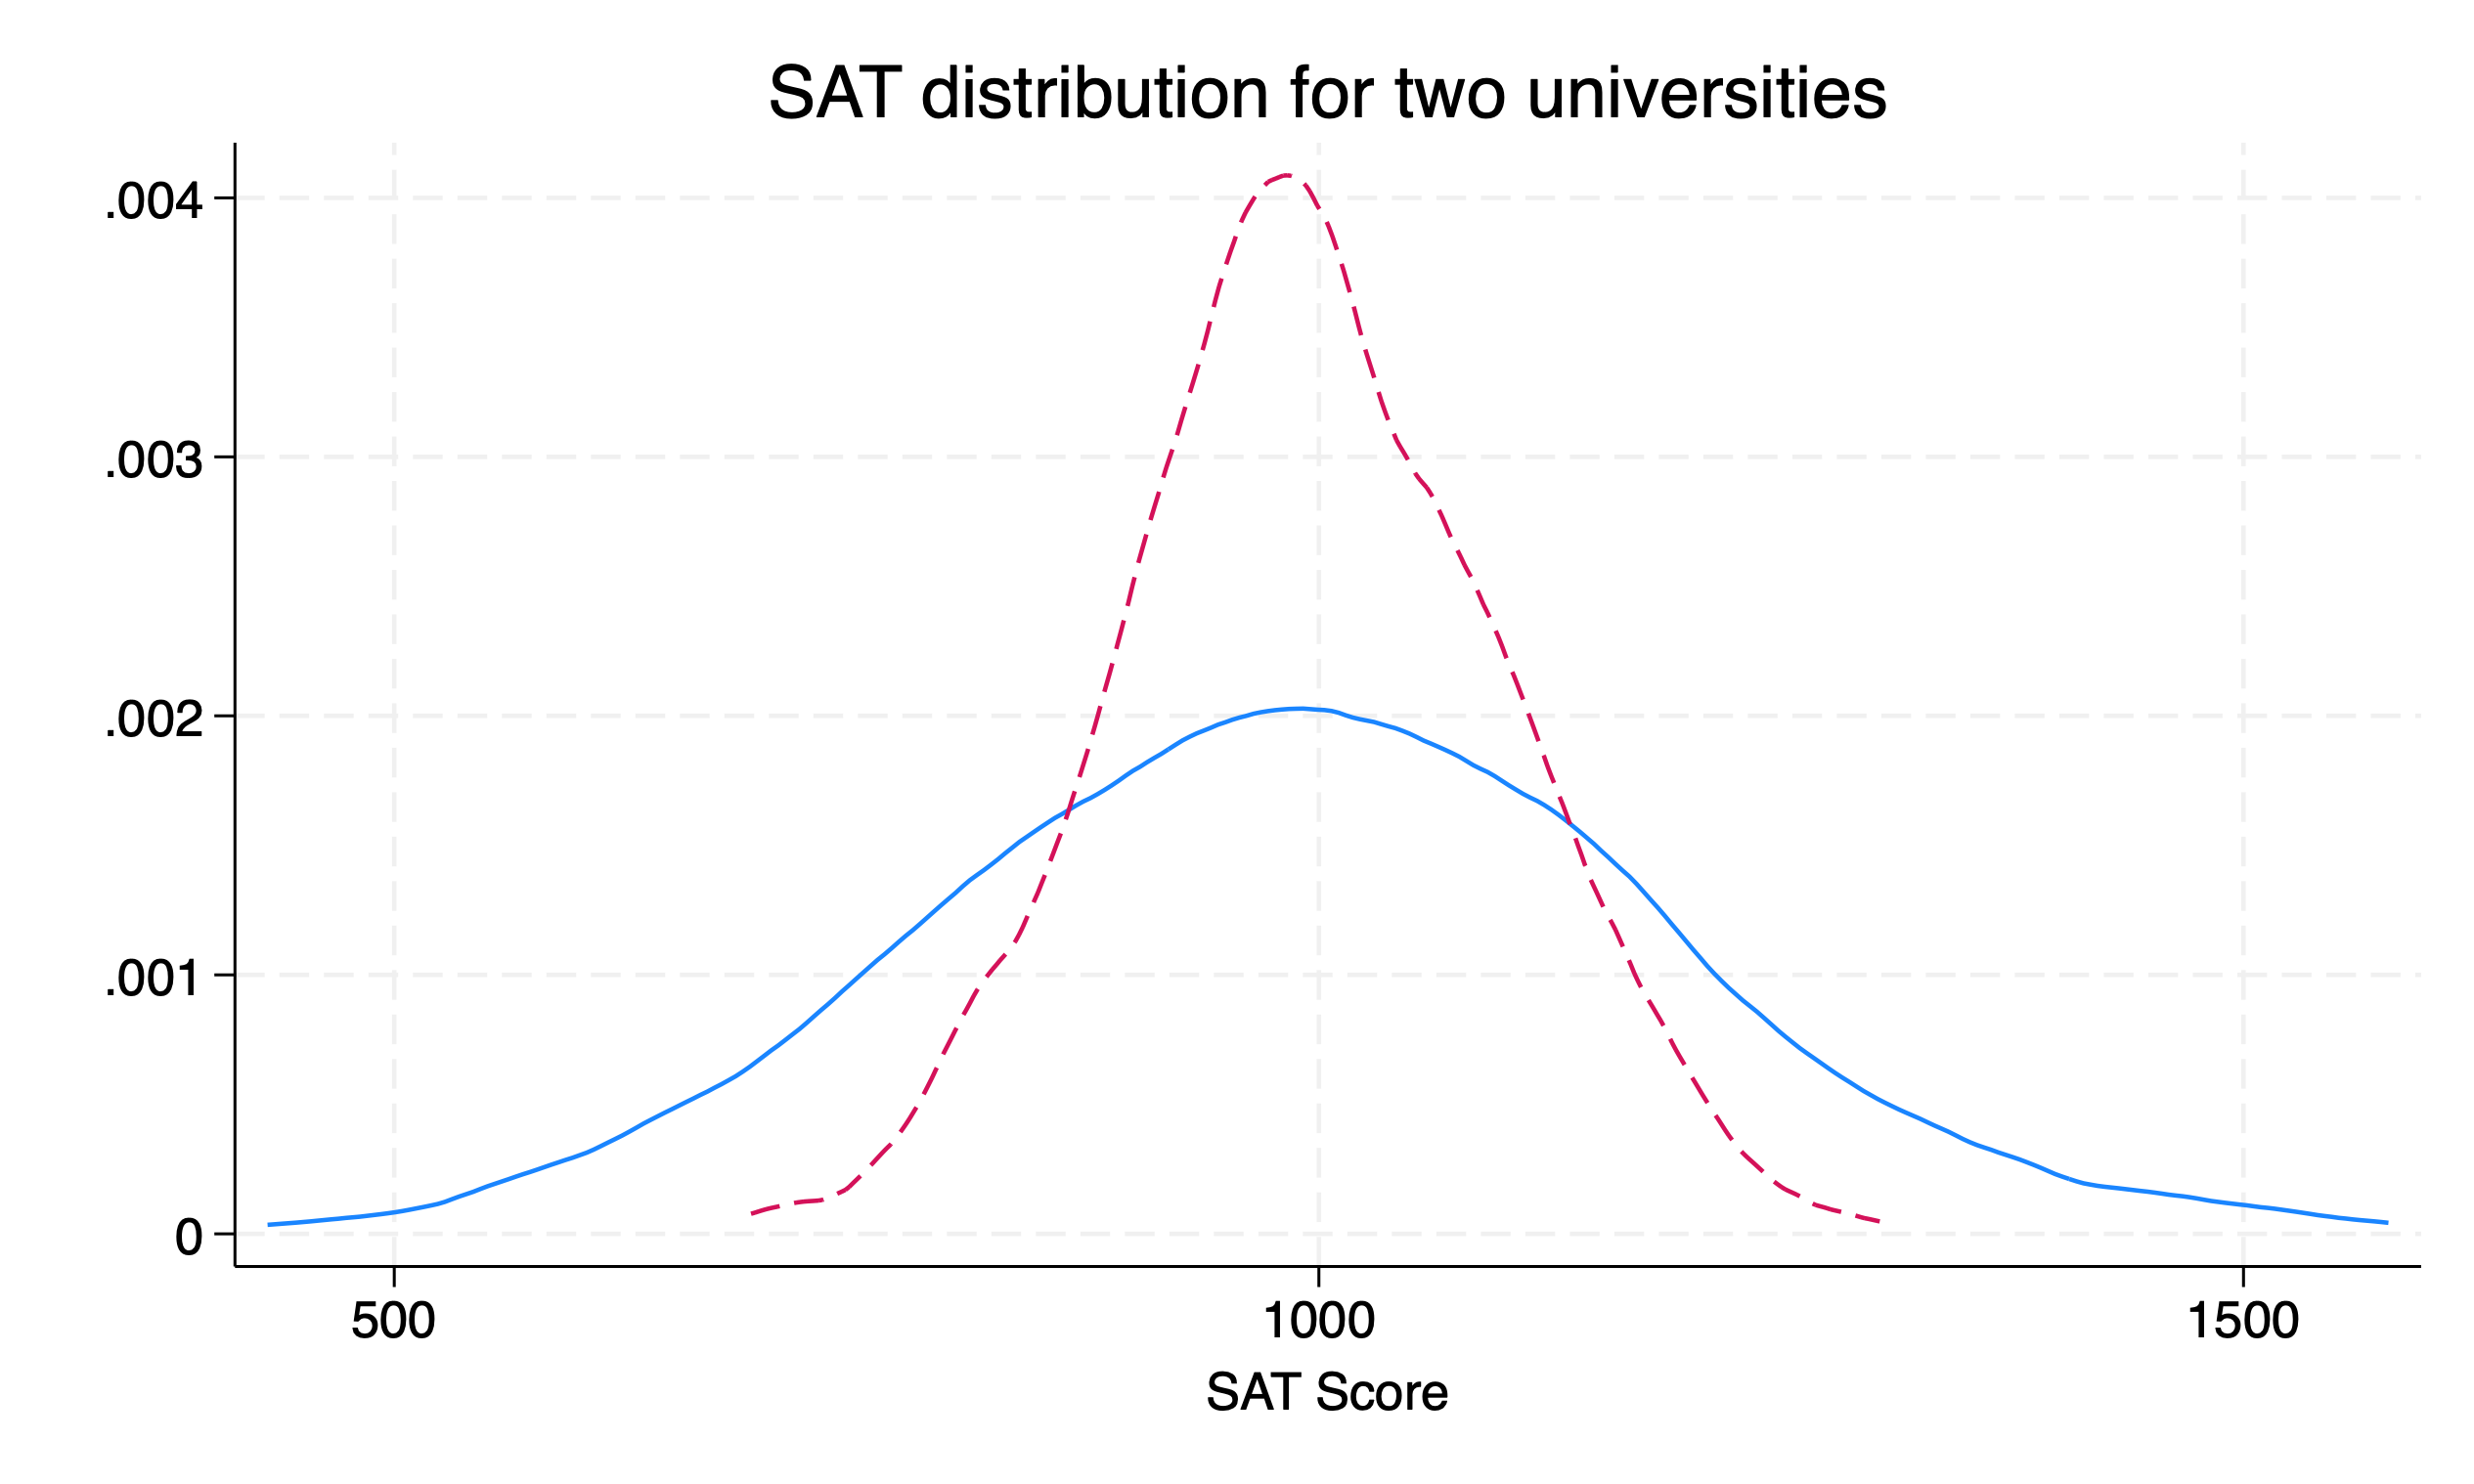
\includegraphics[keepaspectratio,alt={Figure 5.2. Distributions with same M = 1000 but SDs = 100 or 200}]{week3_figure5_2.png}}
\caption{Figure 5.2. Distributions with same \(M = 1000\) but \(SDs = 100\) or \(200\)}
\end{figure}

Both are normally distributed and have idential means \(\mu=1000\), but the university with a smaller \(SD\) has a distribution tightly packed around mean. The other distribution of SAT scores is much more dispersed around the mean.

\section{Nominal (Unordered) Categories}\label{nominal-unordered-categories}

Nominal categorical variable do not have a natural order. Examples include ethnicity, sex, martial status, car color, food categories, etc. To summarize a unordered, nominal categorical variable is to utilize frequencies and the mode. We will use the ``descriptive\_gss.dta'' dataset.

\subsection{Frequenices}\label{frequenices}

The \emph{tabulate} command can be used to get frequencies of distributions for sex and marital status. Acock uses polviews as well, but I would agrue that there can be a clear order to political views.

Please note that the \emph{tabulate} command for one-way tabulation can take one variable at a time. If we add two variables, we will conducte a two-way tabulation. If we want to conduct multiple one-way tabulations on one line, we can use the \emph{tab1} command. Please note that \emph{tab2} will conduct two-way tabulation of all combinations of variable included.

\begin{Shaded}
\begin{Highlighting}[]
\KeywordTok{use}\NormalTok{ descriptive\_gss, }\KeywordTok{clear}
\KeywordTok{tabulate}\NormalTok{ sex}

\KeywordTok{tab1}\NormalTok{ sex martial}
\end{Highlighting}
\end{Shaded}

\begin{verbatim}
respondents |
        sex |      Freq.     Percent        Cum.
------------+-----------------------------------
       male |      1,228       44.41       44.41
     female |      1,537       55.59      100.00
------------+-----------------------------------
      Total |      2,765      100.00


-> tabulation of sex  

respondents |
        sex |      Freq.     Percent        Cum.
------------+-----------------------------------
       male |      1,228       44.41       44.41
     female |      1,537       55.59      100.00
------------+-----------------------------------
      Total |      2,765      100.00

-> tabulation of marital  

      marital |
       status |      Freq.     Percent        Cum.
--------------+-----------------------------------
      married |      1,269       45.90       45.90
      widowed |        247        8.93       54.83
     divorced |        445       16.09       70.92
    separated |         96        3.47       74.39
never married |        708       25.61      100.00
--------------+-----------------------------------
        Total |      2,765      100.00
\end{verbatim}

If we use the \emph{tabulate} command with both marital and sex, we will calculate a two-way tabulation.

\begin{Shaded}
\begin{Highlighting}[]
\KeywordTok{use}\NormalTok{ descriptive\_gss, }\KeywordTok{clear}
\KeywordTok{tabulate}\NormalTok{ sex martial}
\end{Highlighting}
\end{Shaded}

\begin{verbatim}
respondent |                     marital status
     s sex |   married    widowed   divorced  separated  never mar |     Total
-----------+-------------------------------------------------------+----------
      male |       613         46        191         33        345 |     1,228 
    female |       656        201        254         63        363 |     1,537 
-----------+-------------------------------------------------------+----------
     Total |     1,269        247        445         96        708 |     2,765 
\end{verbatim}

Let's take a look polviews.

\begin{Shaded}
\begin{Highlighting}[]
\NormalTok{tabuate polviews}
\end{Highlighting}
\end{Shaded}

\begin{verbatim}
    think of self as |
          liberal or |
        conservative |      Freq.     Percent        Cum.
---------------------+-----------------------------------
   extremely liberal |         47        3.53        3.53
             liberal |        143       10.74       14.27
    slightly liberal |        159       11.95       26.22
            moderate |        522       39.22       65.44
slghtly conservative |        209       15.70       81.14
        conservative |        210       15.78       96.92
extrmly conservative |         41        3.08      100.00
---------------------+-----------------------------------
               Total |      1,331      100.00
\end{verbatim}

I would agrue that there is a clear natural order to this variable.

Ben Jann in 2007 provided a revision of \emph{tab1} called \emph{fre}. We can install his command using the \emph{ssc install} command. The output from the \emph{fre} command is a bit easier to read compared to tab1

\begin{Shaded}
\begin{Highlighting}[]
\KeywordTok{ssc}\NormalTok{ install fre}
\end{Highlighting}
\end{Shaded}

\begin{Shaded}
\begin{Highlighting}[]
\NormalTok{fre sex martial}
\end{Highlighting}
\end{Shaded}

\begin{verbatim}
sex -- respondents sex
--------------------------------------------------------------
                 |      Freq.    Percent      Valid       Cum.
-----------------+--------------------------------------------
Valid   1 male   |       1228      44.41      44.41      44.41
        2 female |       1537      55.59      55.59     100.00
        Total    |       2765     100.00     100.00           
--------------------------------------------------------------

marital -- marital status
---------------------------------------------------------------------
                        |      Freq.    Percent      Valid       Cum.
------------------------+--------------------------------------------
Valid   1 married       |       1269      45.90      45.90      45.90
        2 widowed       |        247       8.93       8.93      54.83
        3 divorced      |        445      16.09      16.09      70.92
        4 separated     |         96       3.47       3.47      74.39
        5 never married |        708      25.61      25.61     100.00
        Total           |       2765     100.00     100.00           
---------------------------------------------------------------------

polviews -- think of self as liberal or conservative
----------------------------------------------------------------------------
                               |      Freq.    Percent      Valid       Cum.
-------------------------------+--------------------------------------------
Valid   1 extremely liberal    |         47       1.70       3.53       3.53
        2 liberal              |        143       5.17      10.74      14.27
        3 slightly liberal     |        159       5.75      11.95      26.22
        4 moderate             |        522      18.88      39.22      65.44
        5 slghtly conservative |        209       7.56      15.70      81.14
        6 conservative         |        210       7.59      15.78      96.92
        7 extrmly conservative |         41       1.48       3.08     100.00
        Total                  |       1331      48.14     100.00           
Missing .                      |       1434      51.86                      
Total                          |       2765     100.00                      
----------------------------------------------------------------------------
\end{verbatim}

\subsection{Pie Charts}\label{pie-charts}

\textbf{DO NOT USE PIE CHARTS!}

There is no reason to use a pie chart when you can use a bar chart.

For pedagologic purposes only, you can create a pie chart with the \emph{graph pie} command. Please do not use this.

\begin{Shaded}
\begin{Highlighting}[]
\KeywordTok{graph}\NormalTok{ pie, }\BaseNTok{over}\NormalTok{(marital) cw }\KeywordTok{sort}\NormalTok{(marital) }\CommentTok{///}
    \BaseNTok{title}\NormalTok{(Marital status }\KeywordTok{in}\NormalTok{ the United States) }\KeywordTok{note}\NormalTok{(descriptive\_gss.dta) }\CommentTok{///}
    \DecValTok{scheme}\NormalTok{(s2color)}
\end{Highlighting}
\end{Shaded}

\begin{figure}
\centering
\pandocbounded{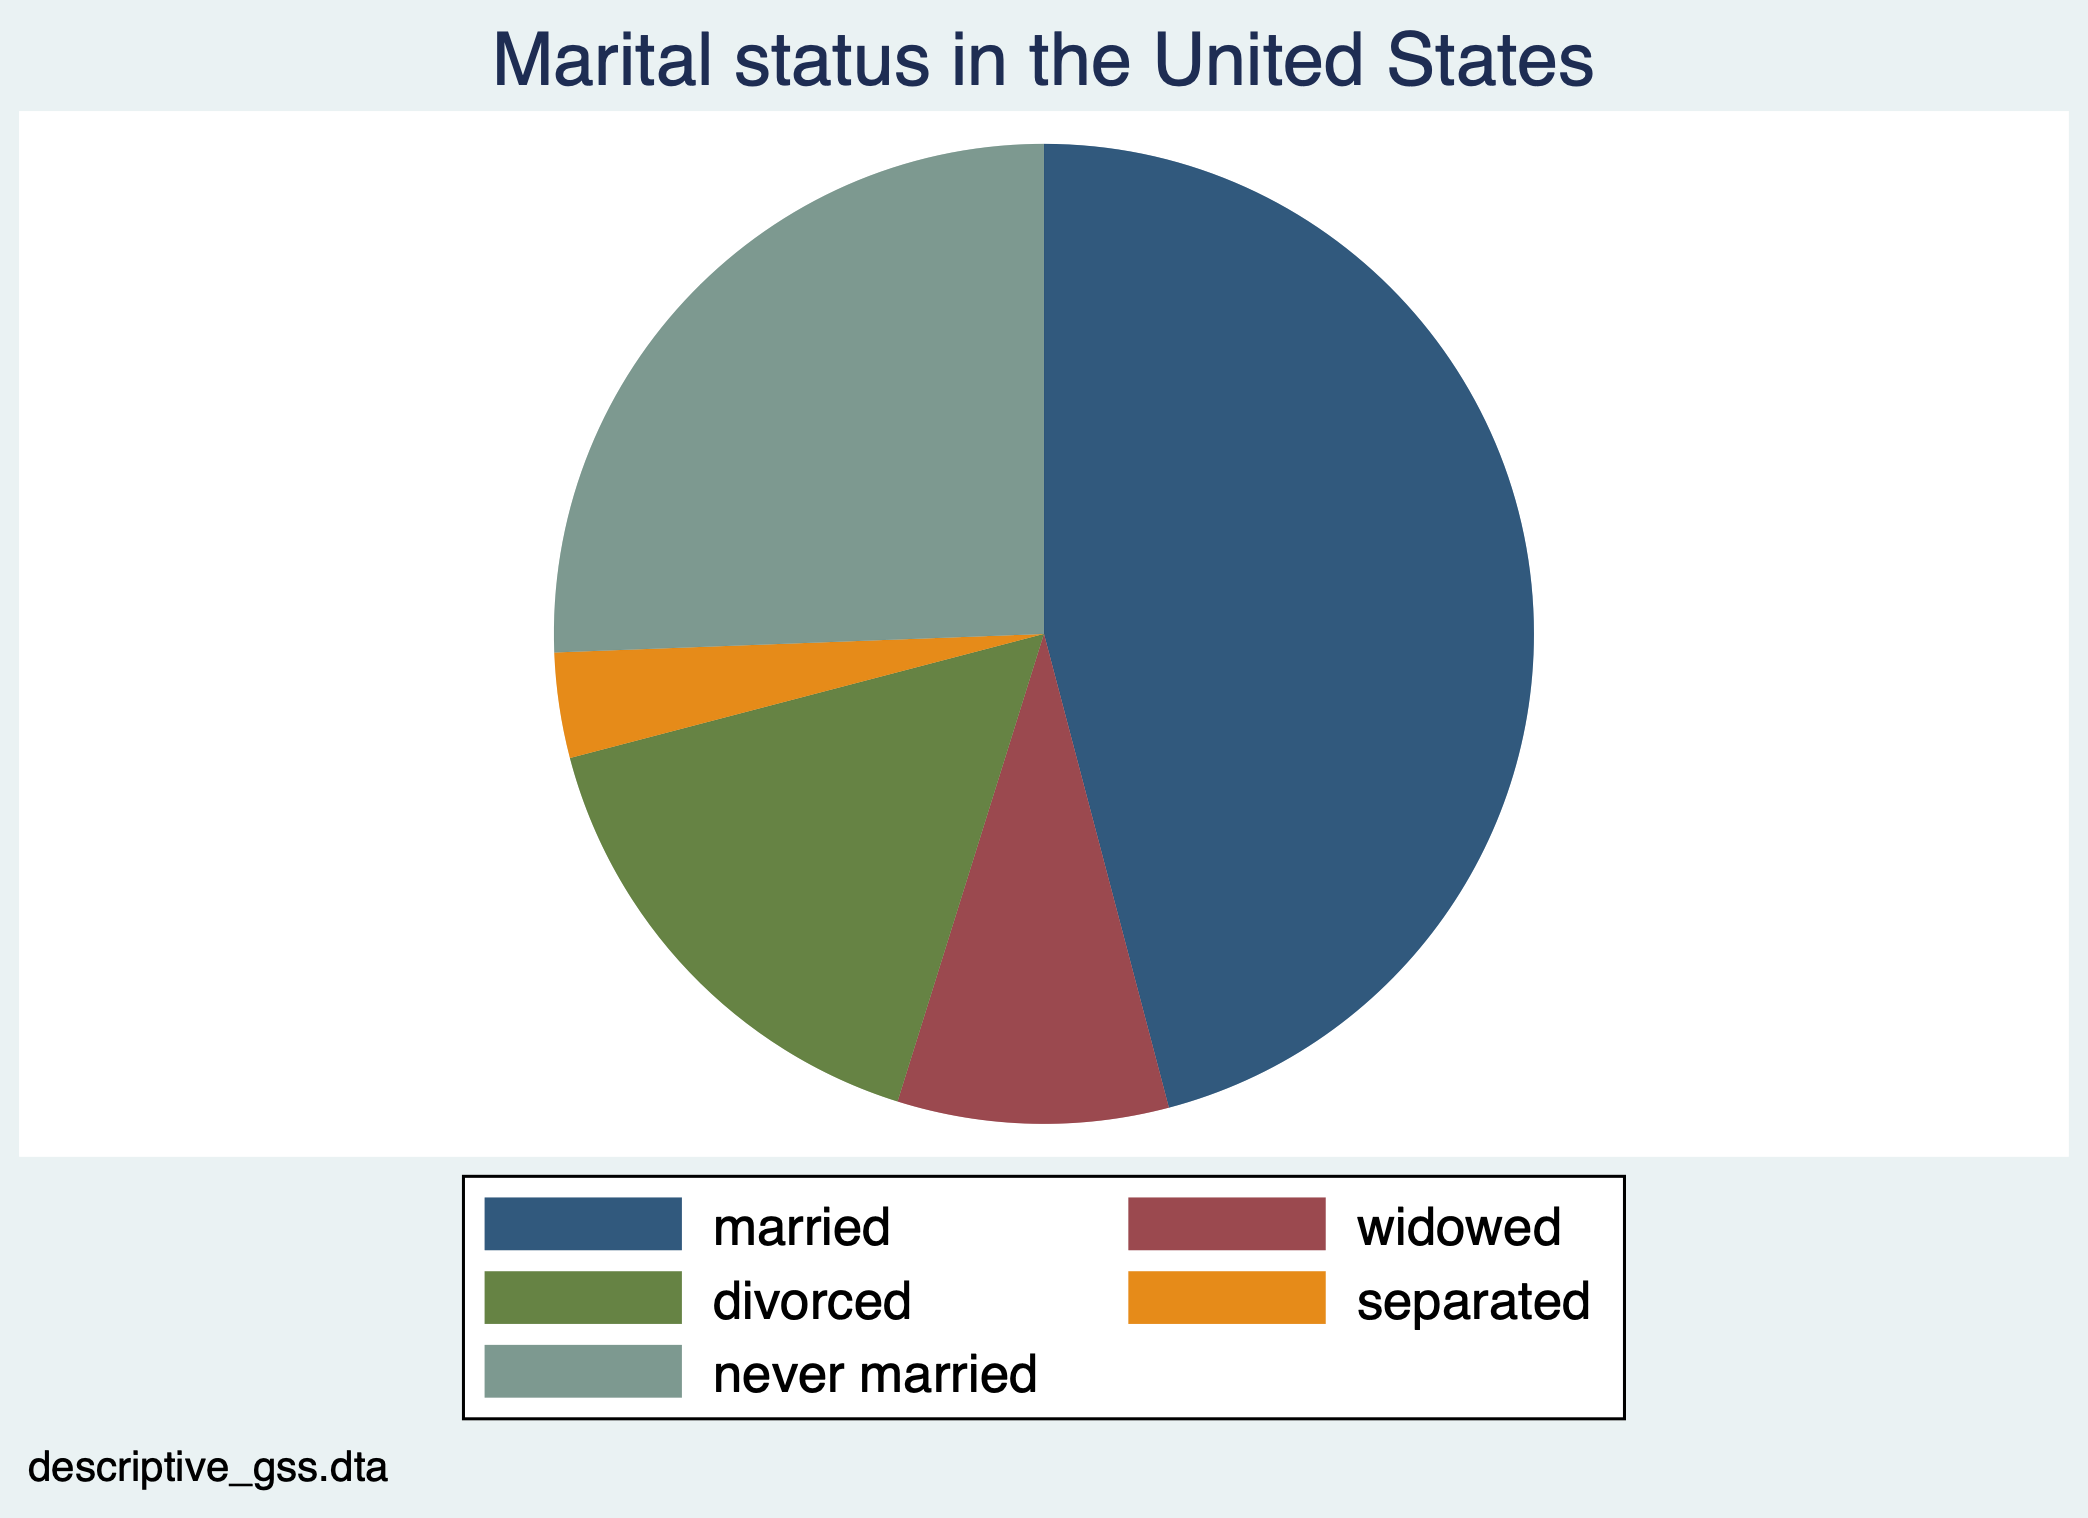
\includegraphics[keepaspectratio,alt={Figure 5.5: Pie Chart of marital status in the U.S.}]{week3_pie.png}}
\caption{Figure 5.5: Pie Chart of marital status in the U.S.}
\end{figure}

What I do want to bring to your attention is the options \emph{title}, \emph{note}, and \emph{scheme}. We can add a title to the graph, a caption note, and a color scheme.

\subsection{Bar Charts}\label{bar-charts}

To display frequencies of nomimal variables, we should use bar charts. We have a couple of options with \emph{graph bar}. We can display frequencies or we can display percentages.

First, we can use a bar chart with frequencies. We will use the \emph{graph bar} command. However, we will not enter \emph{graph bar marital}. What we need to do is add \emph{(count)} for frequencies and the option \emph{over(var)}. We will also want to label the data with the option \emph{blabel(bar, format(\%9.2f))}

\begin{Shaded}
\begin{Highlighting}[]
\KeywordTok{graph} \BaseNTok{bar}\NormalTok{ (}\FunctionTok{count}\NormalTok{), }\BaseNTok{over}\NormalTok{(marital) }\DecValTok{scheme}\NormalTok{(s2color) }\BaseNTok{blabel}\NormalTok{(}\BaseNTok{bar}\NormalTok{, }\KeywordTok{format}\NormalTok{(\%9.0f)) }\BaseNTok{title}\NormalTok{(}\StringTok{"Marital status in the United States"}\NormalTok{) }\KeywordTok{note}\NormalTok{(}\StringTok{"descriptive\_gss.dta"}\NormalTok{)}
\end{Highlighting}
\end{Shaded}

\begin{figure}
\centering
\pandocbounded{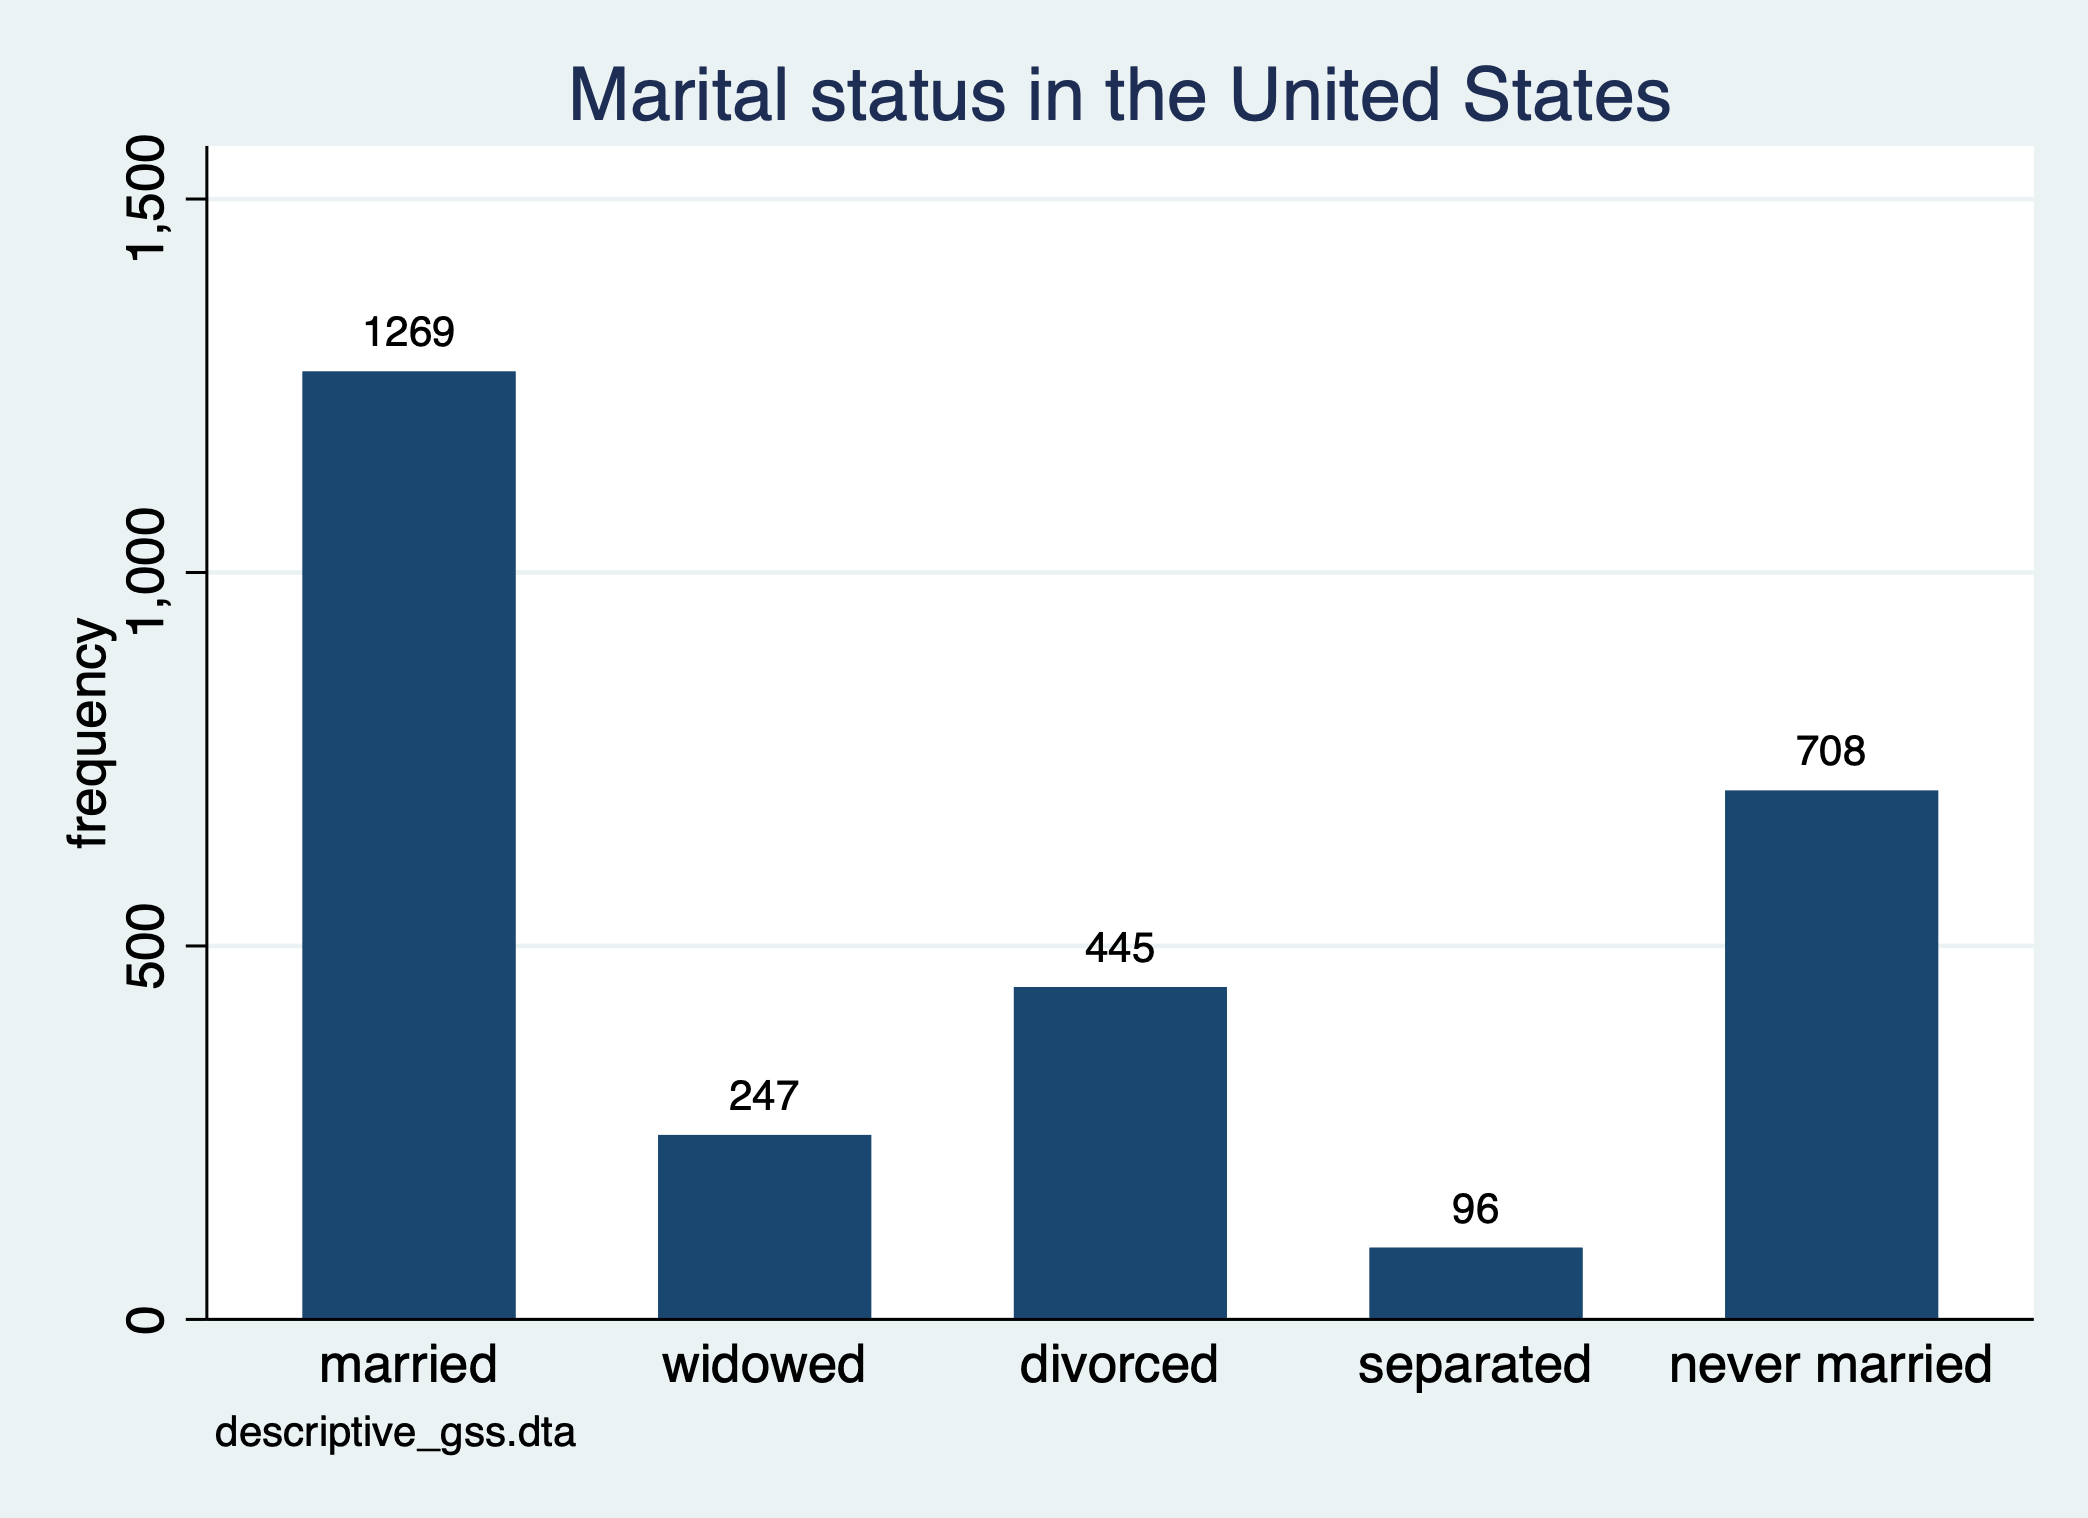
\includegraphics[keepaspectratio,alt={Figure 5.10: Bar chart of marital status of U.S. adults}]{week3_bartotal.png}}
\caption{Figure 5.10: Bar chart of marital status of U.S. adults}
\end{figure}

We can create a similar bar chart, but we will used percentages instead of frequencies. In order to create this type of chart we do not add \emph{(count)} to the \emph{graph bar} command.

\begin{Shaded}
\begin{Highlighting}[]
\KeywordTok{graph} \BaseNTok{bar}\NormalTok{, }\BaseNTok{over}\NormalTok{(marital) }\DecValTok{scheme}\NormalTok{(s2mono) }\BaseNTok{blabel}\NormalTok{(}\BaseNTok{bar}\NormalTok{, }\KeywordTok{format}\NormalTok{(\%9.2f)) }\BaseNTok{title}\NormalTok{(}\StringTok{"Marital status in the United States"}\NormalTok{) }\KeywordTok{note}\NormalTok{(}\StringTok{"descriptive\_gss.dta"}\NormalTok{)}
\end{Highlighting}
\end{Shaded}

\begin{figure}
\centering
\pandocbounded{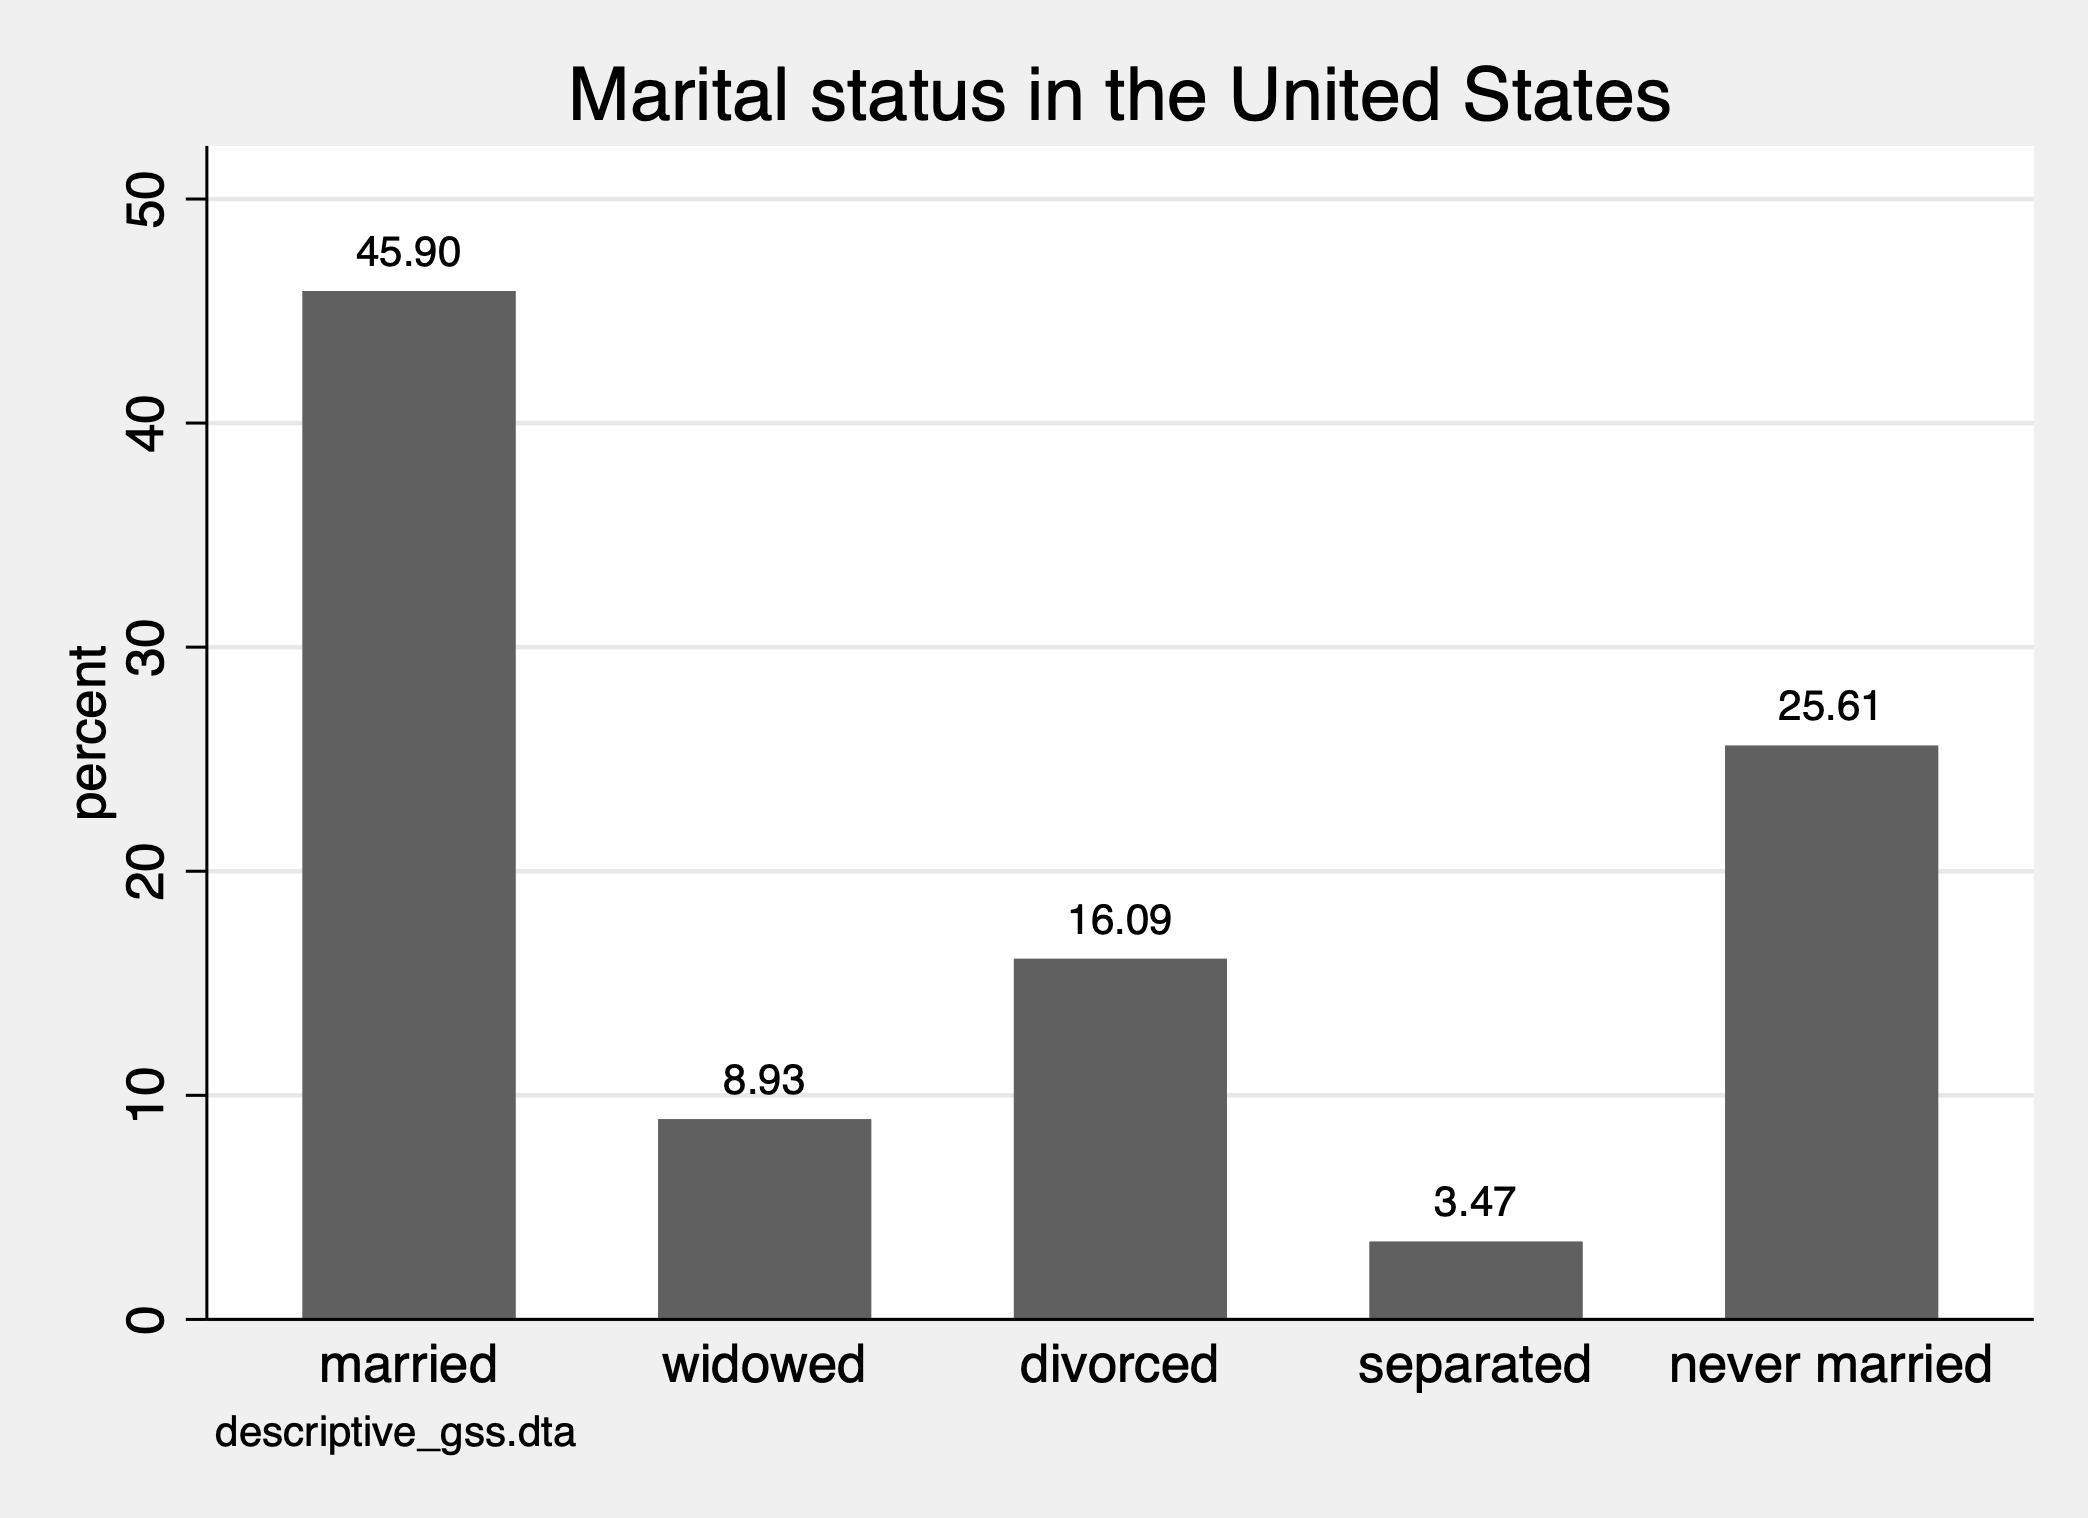
\includegraphics[keepaspectratio,alt={Figure 5.11: Bar chart of marital status of U.S. adults}]{week3_barpct.png}}
\caption{Figure 5.11: Bar chart of marital status of U.S. adults}
\end{figure}

We can actually use histograms with the option \emph{discrete}. Additional options for formatting are provided. \emph{percentage} converts the two-decimal y-axis into two digit whole numbers. \emph{gap} option increases the shape between bars.\emph{addlabel} add values over the bars. \emph{xlabel} add values to the x-axis.

\begin{Shaded}
\begin{Highlighting}[]
\KeywordTok{histogram}\NormalTok{ marital, discrete }\KeywordTok{percent}\NormalTok{ gap(10) addlabel }\KeywordTok{xlabel}\NormalTok{(, valuelabel) }\CommentTok{///}
    \BaseNTok{title}\NormalTok{(Marital status }\KeywordTok{in}\NormalTok{ the United States) }\KeywordTok{note}\NormalTok{(}\StringTok{"descriptive\_gss.dta"}\NormalTok{) }\DecValTok{scheme}\NormalTok{(s2gcolor) }
\end{Highlighting}
\end{Shaded}

\begin{figure}
\centering
\pandocbounded{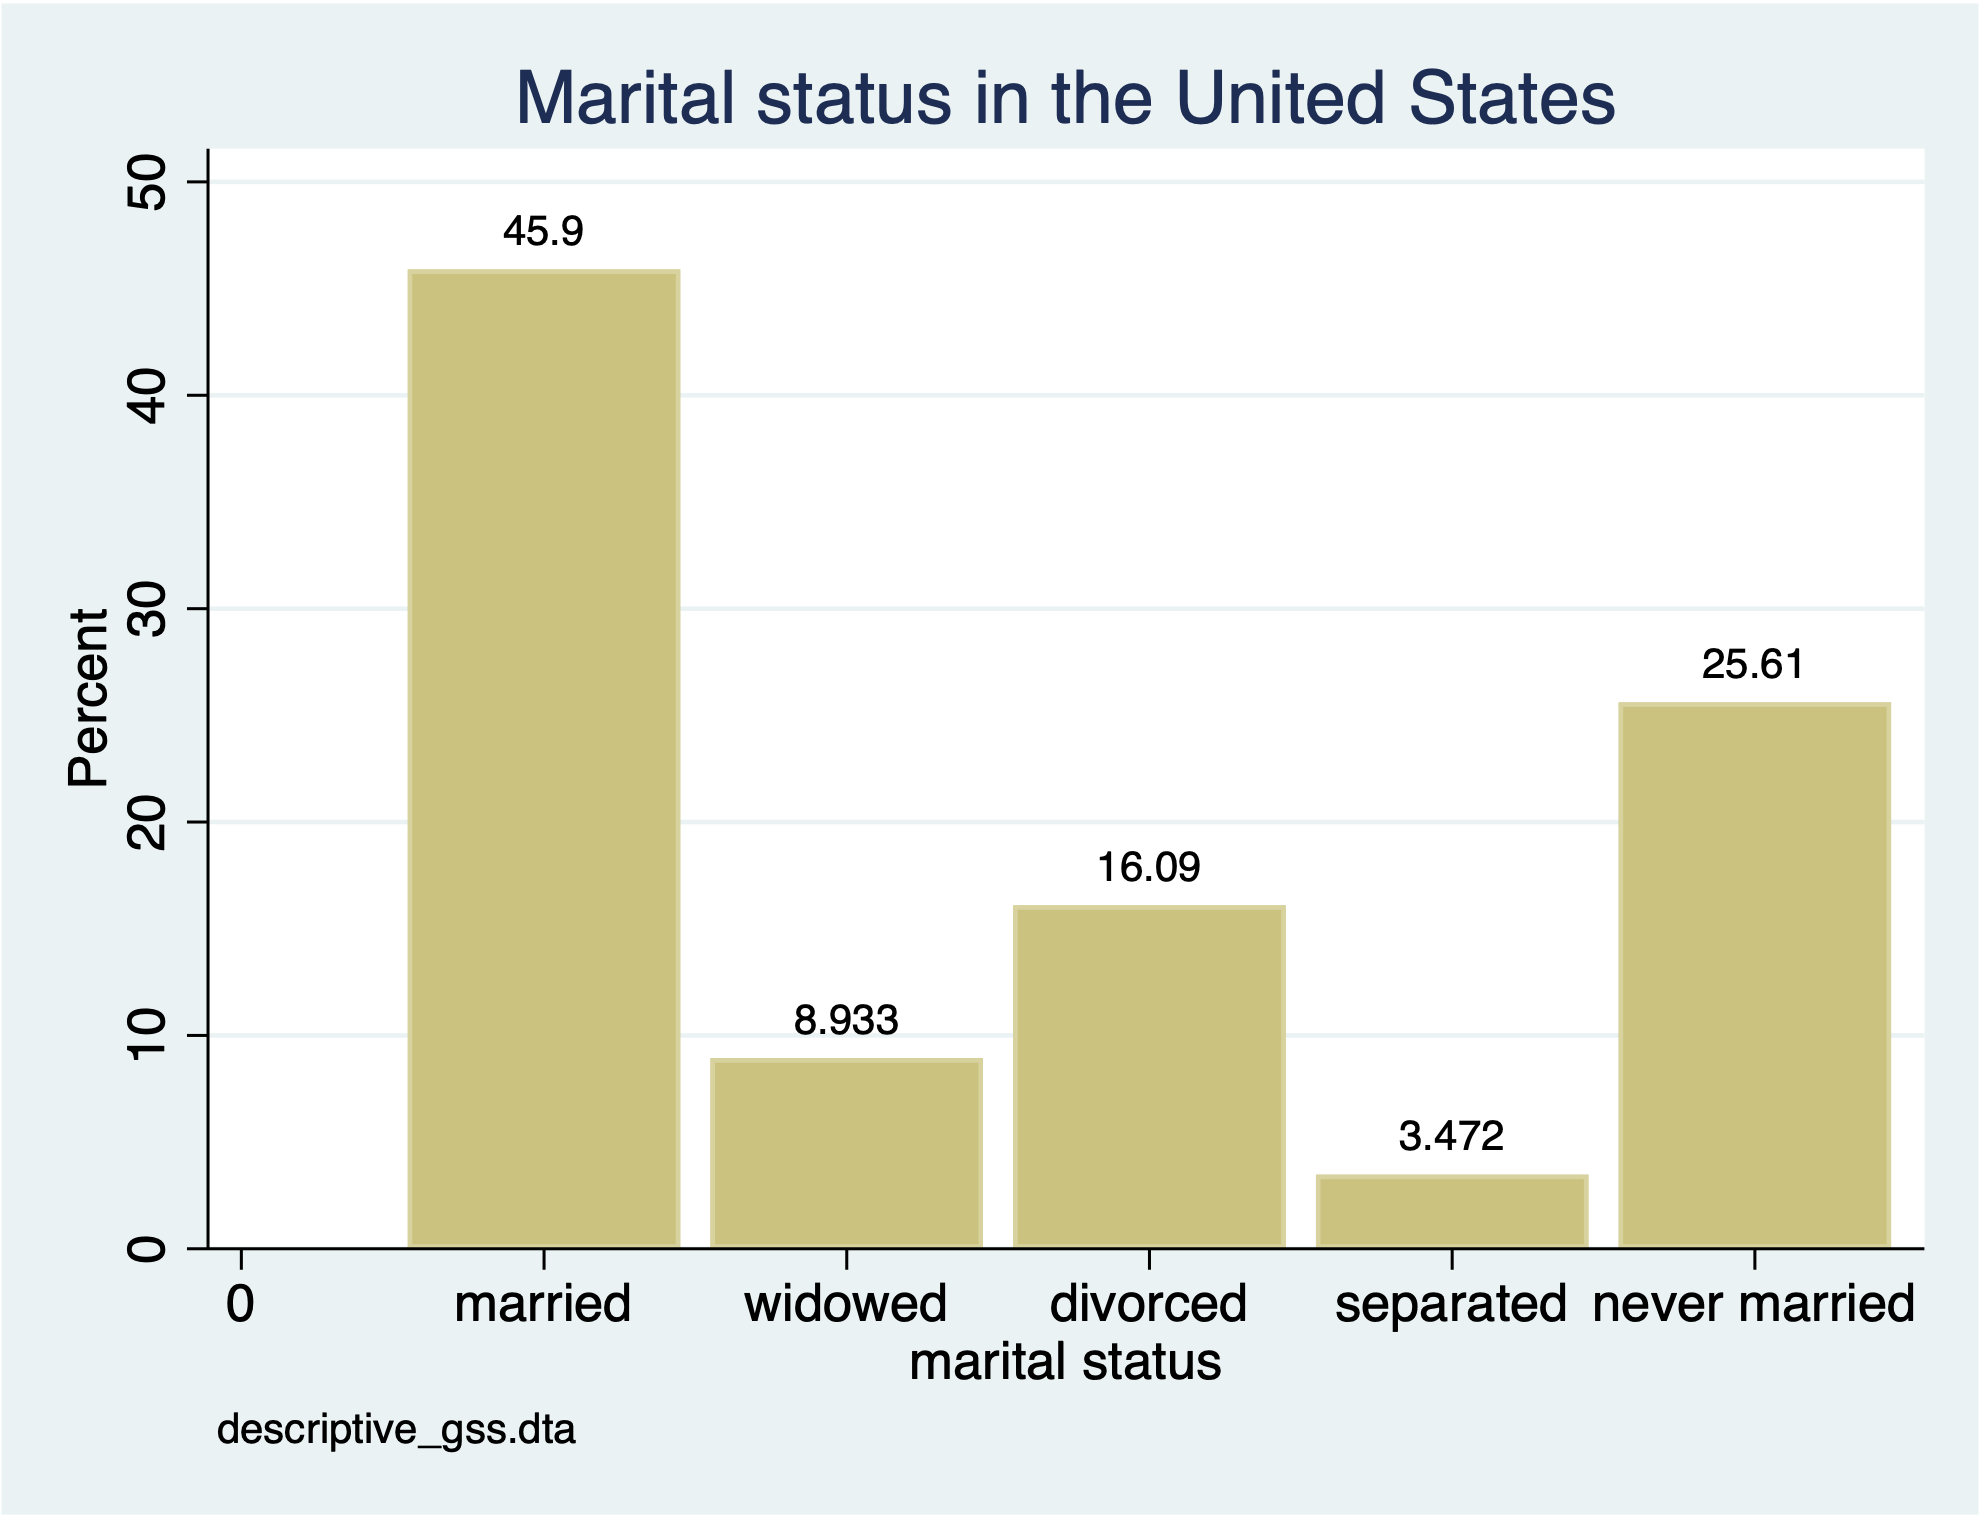
\includegraphics[keepaspectratio,alt={Figure 5.12: Bar chart of marital status of U.S. adults}]{week3_barhist.png}}
\caption{Figure 5.12: Bar chart of marital status of U.S. adults}
\end{figure}

You may have noticed that the prior graph does not produce the frequencies we need. If we will use \emph{histogram} command with the \emph{discrete} option, then we need to add the option \emph{freq} to create a freqency chart with the \emph{histogram} command.

\begin{Shaded}
\begin{Highlighting}[]
\KeywordTok{histogram}\NormalTok{ marital, discrete }\KeywordTok{frequency}\NormalTok{ gap(10) addlabel }\KeywordTok{xlabel}\NormalTok{(, valuelabel) }\CommentTok{///}
    \BaseNTok{title}\NormalTok{(Marital status }\KeywordTok{in}\NormalTok{ the United States) }\KeywordTok{note}\NormalTok{(}\StringTok{"descriptive\_gss.dta"}\NormalTok{) }\DecValTok{scheme}\NormalTok{(sj) }
\end{Highlighting}
\end{Shaded}

\begin{figure}
\centering
\pandocbounded{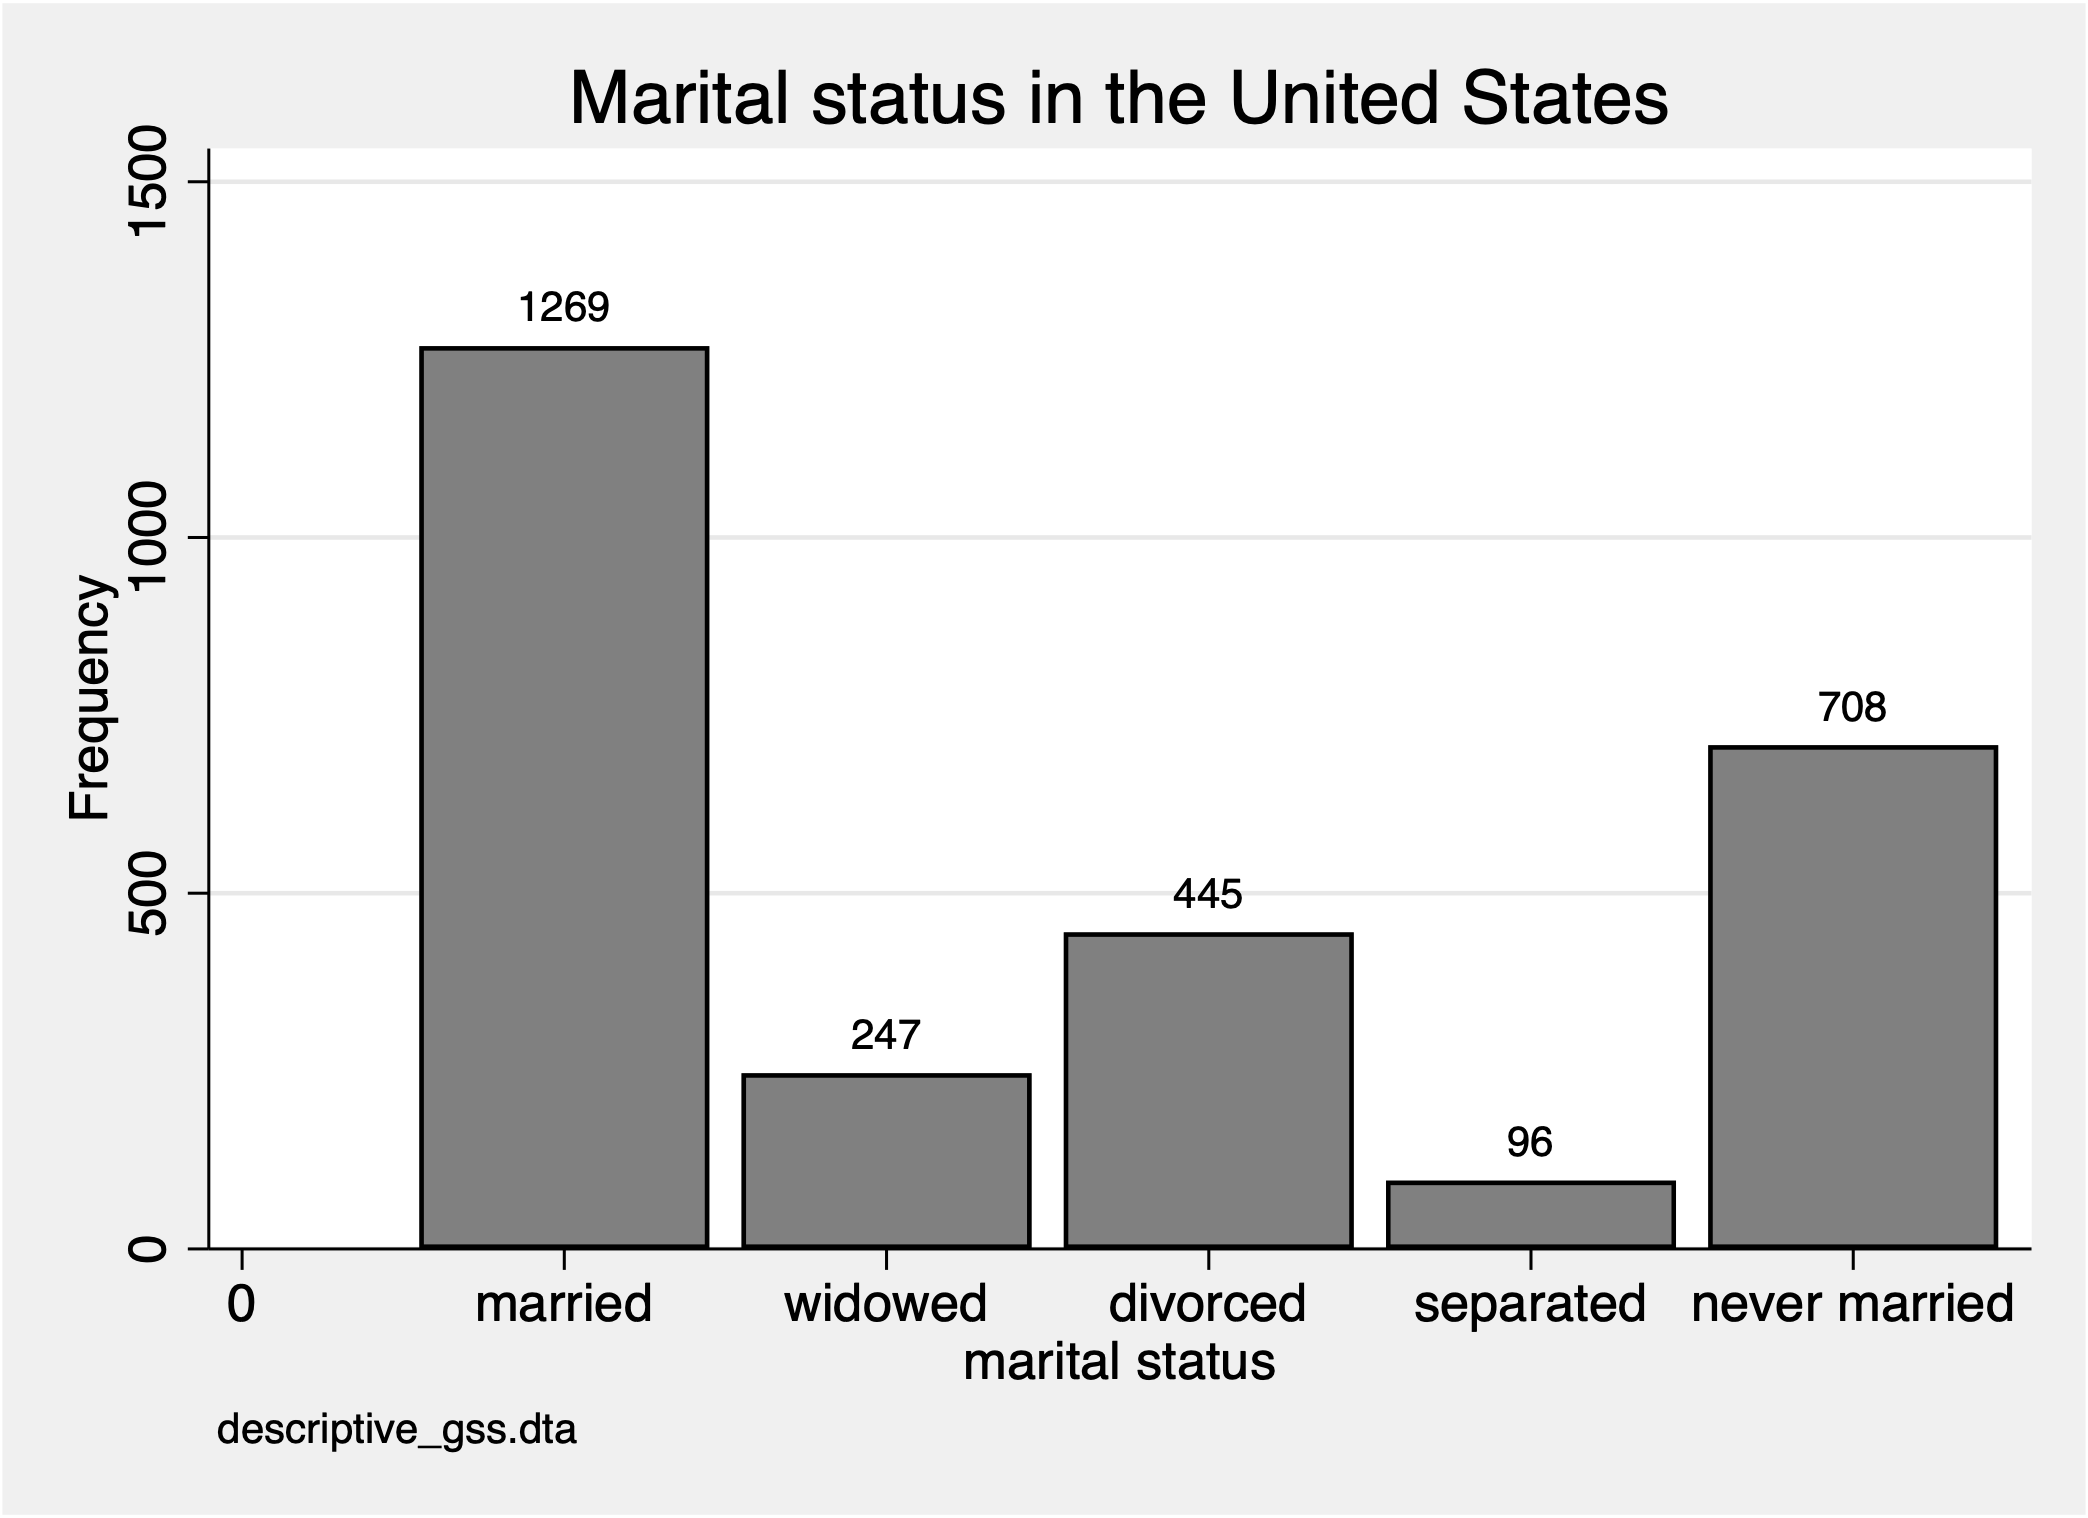
\includegraphics[keepaspectratio,alt={Figure 5.13: Bar chart of marital status of U.S. adults}]{week3_barhistfreq.png}}
\caption{Figure 5.13: Bar chart of marital status of U.S. adults}
\end{figure}

\section{Ordinal Categories}\label{ordinal-categories}

For ordinal categorical variables, we can use mode and median for central tendency. We can calculate the median, or \(50^{th}\) percentile, with the \emph{summarize} command. To get different percentiles, including the median, we need to add the \emph{detail} option.

\begin{Shaded}
\begin{Highlighting}[]
\KeywordTok{sum}\NormalTok{ polviews, }\KeywordTok{detail}
\end{Highlighting}
\end{Shaded}

\begin{verbatim}
          think of self as liberal or conservative
-------------------------------------------------------------
      Percentiles      Smallest
 1%            1              1
 5%            2              1
10%            2              1       Obs               1,331
25%            3              1       Sum of wgt.       1,331

50%            4                      Mean           4.124718
                        Largest       Std. dev.      1.385016
75%            5              7
90%            6              7       Variance       1.918268
95%            6              7       Skewness      -.1509408
99%            7              7       Kurtosis       2.693351
\end{verbatim}

The median value is 4 our of the 1 through 7. What does 4 imply?

We can also use the \emph{tabulate} or \emph{tab1} commands to find the mode and what each value means. If we want to show the value and the value label, we can run the \emph{numlabel} command.

\begin{Shaded}
\begin{Highlighting}[]
\KeywordTok{numlabel} \DataTypeTok{\_all}\NormalTok{, add}
\KeywordTok{tab1}\NormalTok{ polviews}
\end{Highlighting}
\end{Shaded}

\begin{verbatim}
-> tabulation of polviews  

       think of self as |
liberal or conservative |      Freq.     Percent        Cum.
------------------------+-----------------------------------
   1. extremely liberal |         47        3.53        3.53
             2. liberal |        143       10.74       14.27
    3. slightly liberal |        159       11.95       26.22
            4. moderate |        522       39.22       65.44
5. slghtly conservative |        209       15.70       81.14
        6. conservative |        210       15.78       96.92
7. extrmly conservative |         41        3.08      100.00
------------------------+-----------------------------------
                  Total |      1,331      100.00
\end{verbatim}

The mode is 4, which is moderate. So the median and mode are the same for \emph{polviews} variable.

For distribution, we can use the \emph{tabulate} or \emph{tab1} commands and we can use \emph{graph bar (count), over(var)} and \emph{histgram var, discrete freq} commands.

First, we will use a \emph{histogram var, discrete}, but we will change the color scheme.

\begin{Shaded}
\begin{Highlighting}[]
\KeywordTok{histogram}\NormalTok{ polviews, discrete }\KeywordTok{frequency} \BaseNTok{start}\NormalTok{(1) }\CommentTok{///}
   \BaseNTok{title}\NormalTok{(Political views }\KeywordTok{in}\NormalTok{ the United States) }\BaseNTok{subtitle}\NormalTok{(}\KeywordTok{by}\NormalTok{ adult population) }\CommentTok{///}
   \BaseNTok{caption}\NormalTok{(General Social Survey 2002) }\BaseNTok{xtitle}\NormalTok{(Political conservatism) }\DecValTok{scheme}\NormalTok{(economist)}
\end{Highlighting}
\end{Shaded}

\begin{figure}
\centering
\pandocbounded{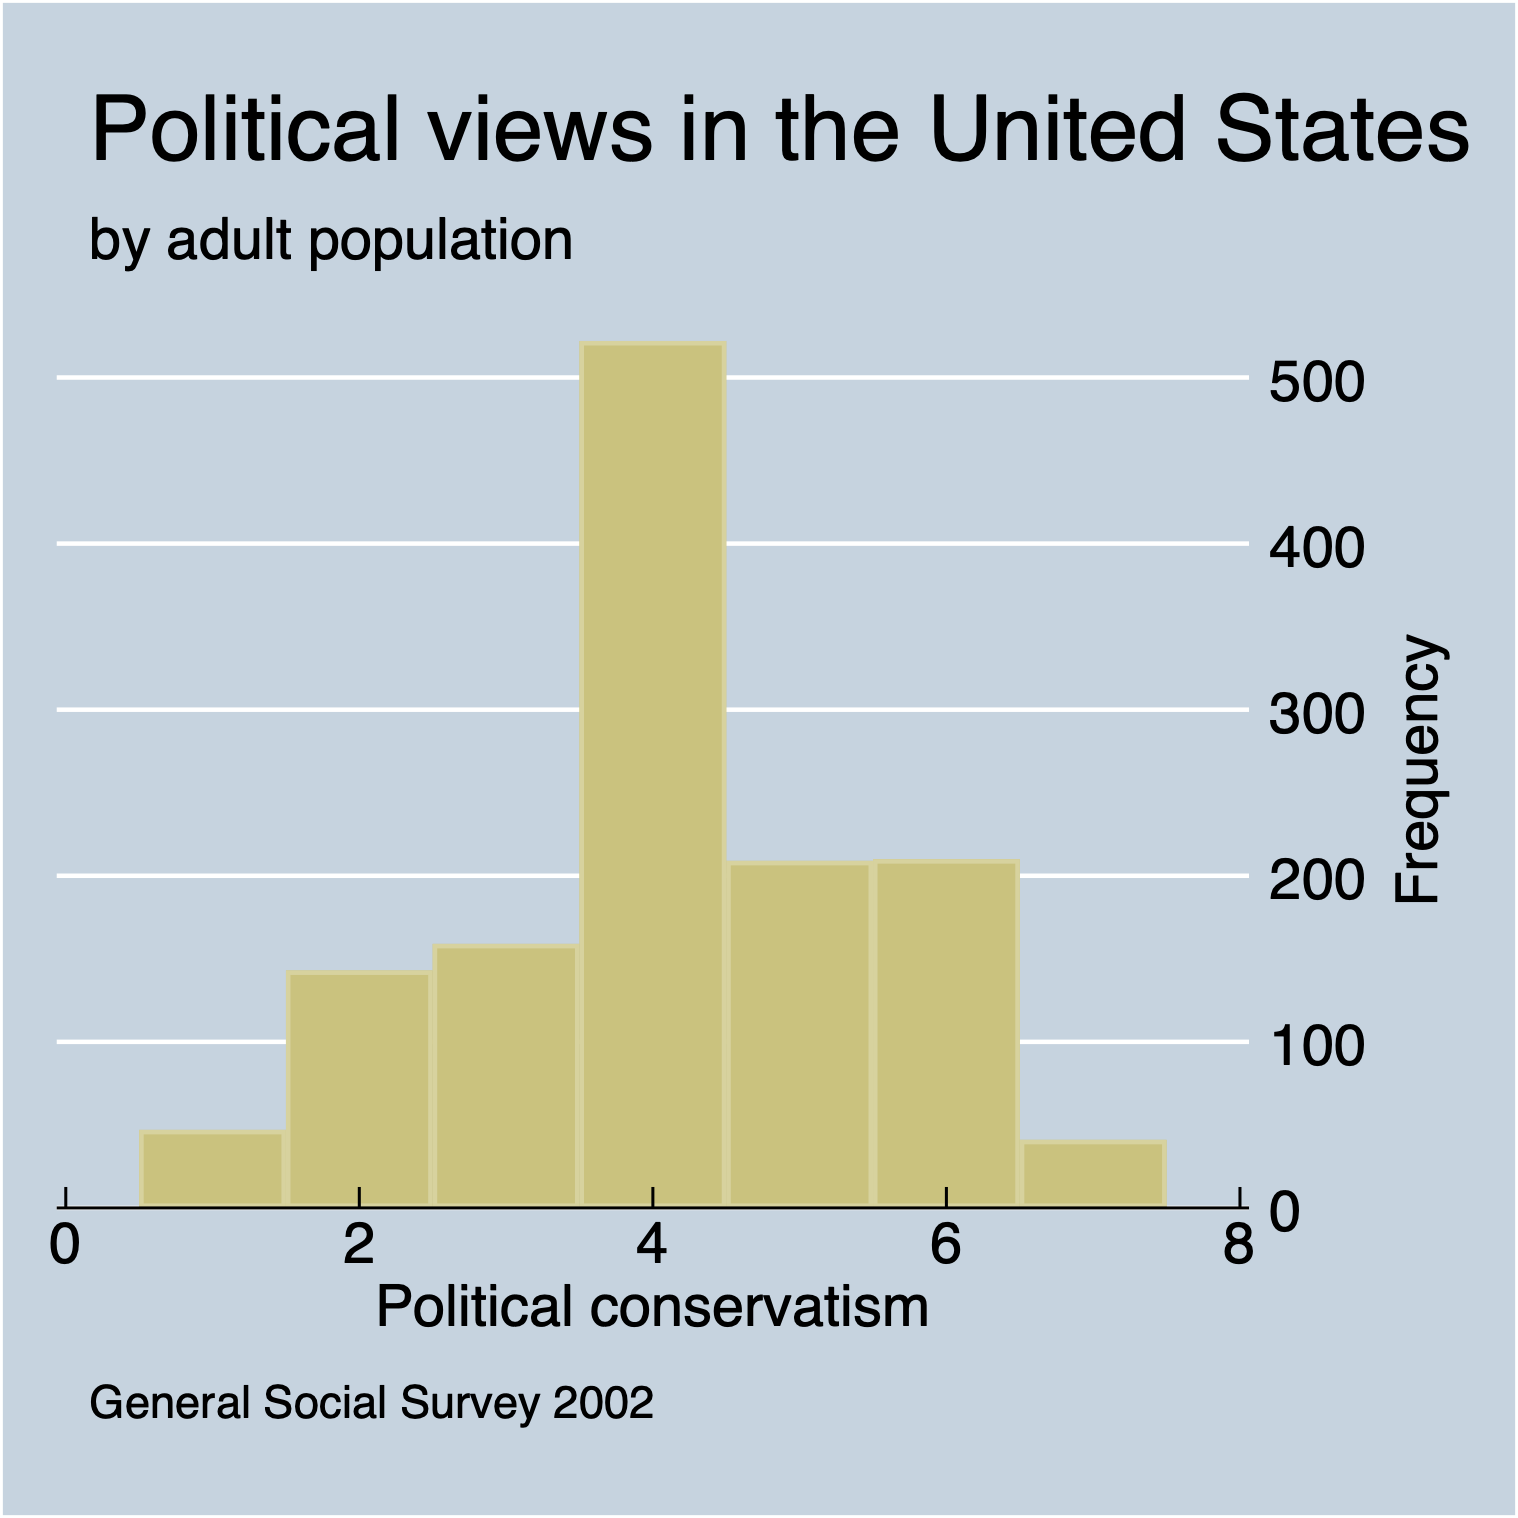
\includegraphics[keepaspectratio,alt={Figure 5.14: Histogram of political views of U.S. adults}]{week3_polhist.png}}
\caption{Figure 5.14: Histogram of political views of U.S. adults}
\end{figure}

Now, we will conduct the same exercise but we will use a horizontal bar chart with the command \emph{graph hbar}.

\begin{Shaded}
\begin{Highlighting}[]
\KeywordTok{graph} \BaseNTok{hbar}\NormalTok{ (}\FunctionTok{count}\NormalTok{), }\BaseNTok{over}\NormalTok{(polviews) }\BaseNTok{title}\NormalTok{(Political views }\KeywordTok{in}\NormalTok{ the United States) }\BaseNTok{subtitle}\NormalTok{(}\KeywordTok{by}\NormalTok{ adult population) }\KeywordTok{note}\NormalTok{(General Social Survey 2002) }\DecValTok{scheme}\NormalTok{(s1mono)}
\end{Highlighting}
\end{Shaded}

\begin{figure}
\centering
\pandocbounded{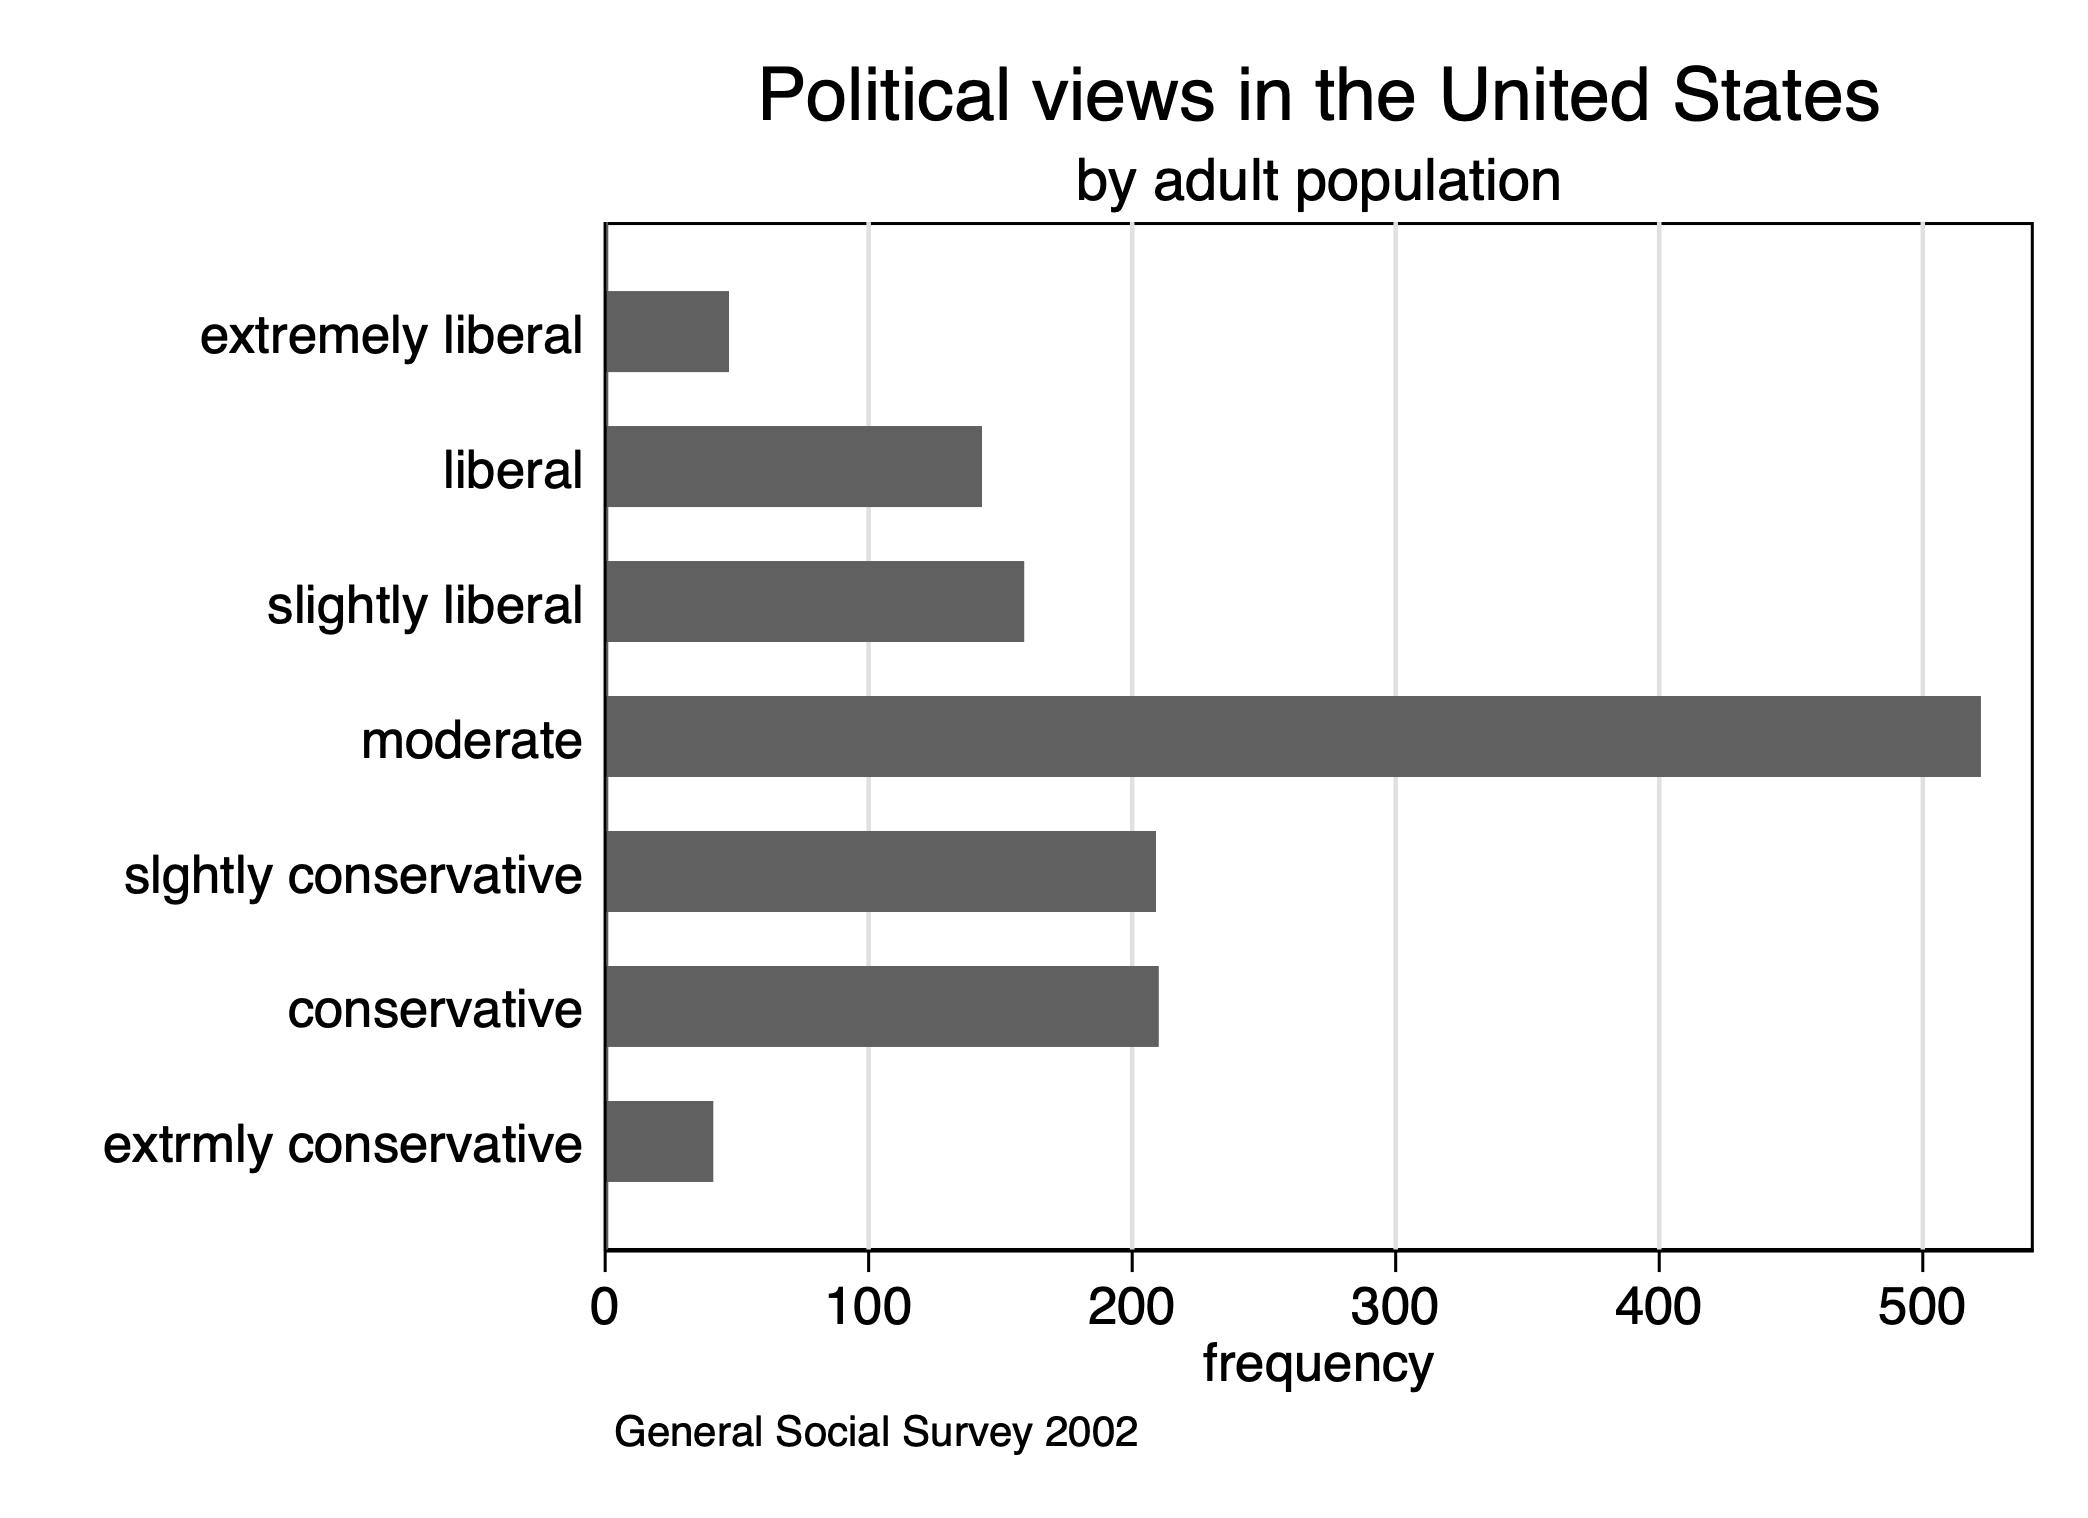
\includegraphics[keepaspectratio,alt={Figure 5.15: Bar Chart of political views of U.S. adults}]{week3_polhbar.png}}
\caption{Figure 5.15: Bar Chart of political views of U.S. adults}
\end{figure}

\section{Quantitative Variables}\label{quantitative-variables}

Our final category is quantitative variables, such as discrete or continuous variables. We will look at the number of hours spent on the internet \emph{wwwhr} and hours worked \emph{hrs1}

For central tendency for these measures, we can use mean, median, and mode. We'll use the \emph{summarize var, detail} command to inspect the mean and median.

\subsection{Summarize and histograms}\label{summarize-and-histograms}

\begin{Shaded}
\begin{Highlighting}[]
\KeywordTok{sum}\NormalTok{ wwwhr, }\KeywordTok{detail}
\KeywordTok{sum}\NormalTok{ hrs1, }\KeywordTok{detail}
\end{Highlighting}
\end{Shaded}

\begin{verbatim}
                     www hours per week
-------------------------------------------------------------
      Percentiles      Smallest
 1%            0              0
 5%            0              0
10%            0              0       Obs               1,574
25%            1              0       Sum of wgt.       1,574

50%            3                      Mean           5.907878
                        Largest       Std. dev.      8.866734
75%            7             60
90%           15             64       Variance       78.61897
95%           21            100       Skewness       3.997908
99%           40            112       Kurtosis       30.39248

              number of hours worked last week
-------------------------------------------------------------
      Percentiles      Smallest
 1%            6              1
 5%           16              2
10%           21              2       Obs               1,729
25%           36              2       Sum of wgt.       1,729

50%           40                      Mean           41.77675
                        Largest       Std. dev.      14.62304
75%           50             89
90%           60             89       Variance       213.8332
95%           68             89       Skewness       .2834814
99%           88             89       Kurtosis       4.310339
\end{verbatim}

For both variables, the median is less than the mean. There is possible skewness, so we can use the command \emph{sktest} to calculate the skewness and kurtosis of the data.

\begin{Shaded}
\begin{Highlighting}[]
\KeywordTok{sktest}\NormalTok{ wwwhr}
\KeywordTok{sktest}\NormalTok{ hrs1}
\end{Highlighting}
\end{Shaded}

\begin{verbatim}
Skewness and kurtosis tests for normality
                                                         ----- Joint test -----
    Variable |       Obs   Pr(skewness)   Pr(kurtosis)   Adj chi2(2)  Prob>chi2
-------------+-----------------------------------------------------------------
       wwwhr |     1,574         0.0000         0.0000       1060.97     0.0000


Skewness and kurtosis tests for normality
                                                         ----- Joint test -----
    Variable |       Obs   Pr(skewness)   Pr(kurtosis)   Adj chi2(2)  Prob>chi2
-------------+-----------------------------------------------------------------
        hrs1 |     1,729         0.0000         0.0000         60.26     0.0000
\end{verbatim}

Based on the skewness of both variables, the probability that \emph{wwwhr} is normal is 0 and the probability that \emph{hrs1} is normal is 0 as well. Based on the kurtosis, the probability that \emph{wwwhr} is normal is 0 and the probability that \emph{hrs1} is normal is 0 as well.

Now we will utilize the \emph{histogram} command to examine the distribution.

\begin{Shaded}
\begin{Highlighting}[]
\KeywordTok{histogram}\NormalTok{ wwwhr, }\KeywordTok{frequency}
\end{Highlighting}
\end{Shaded}

\begin{figure}
\centering
\pandocbounded{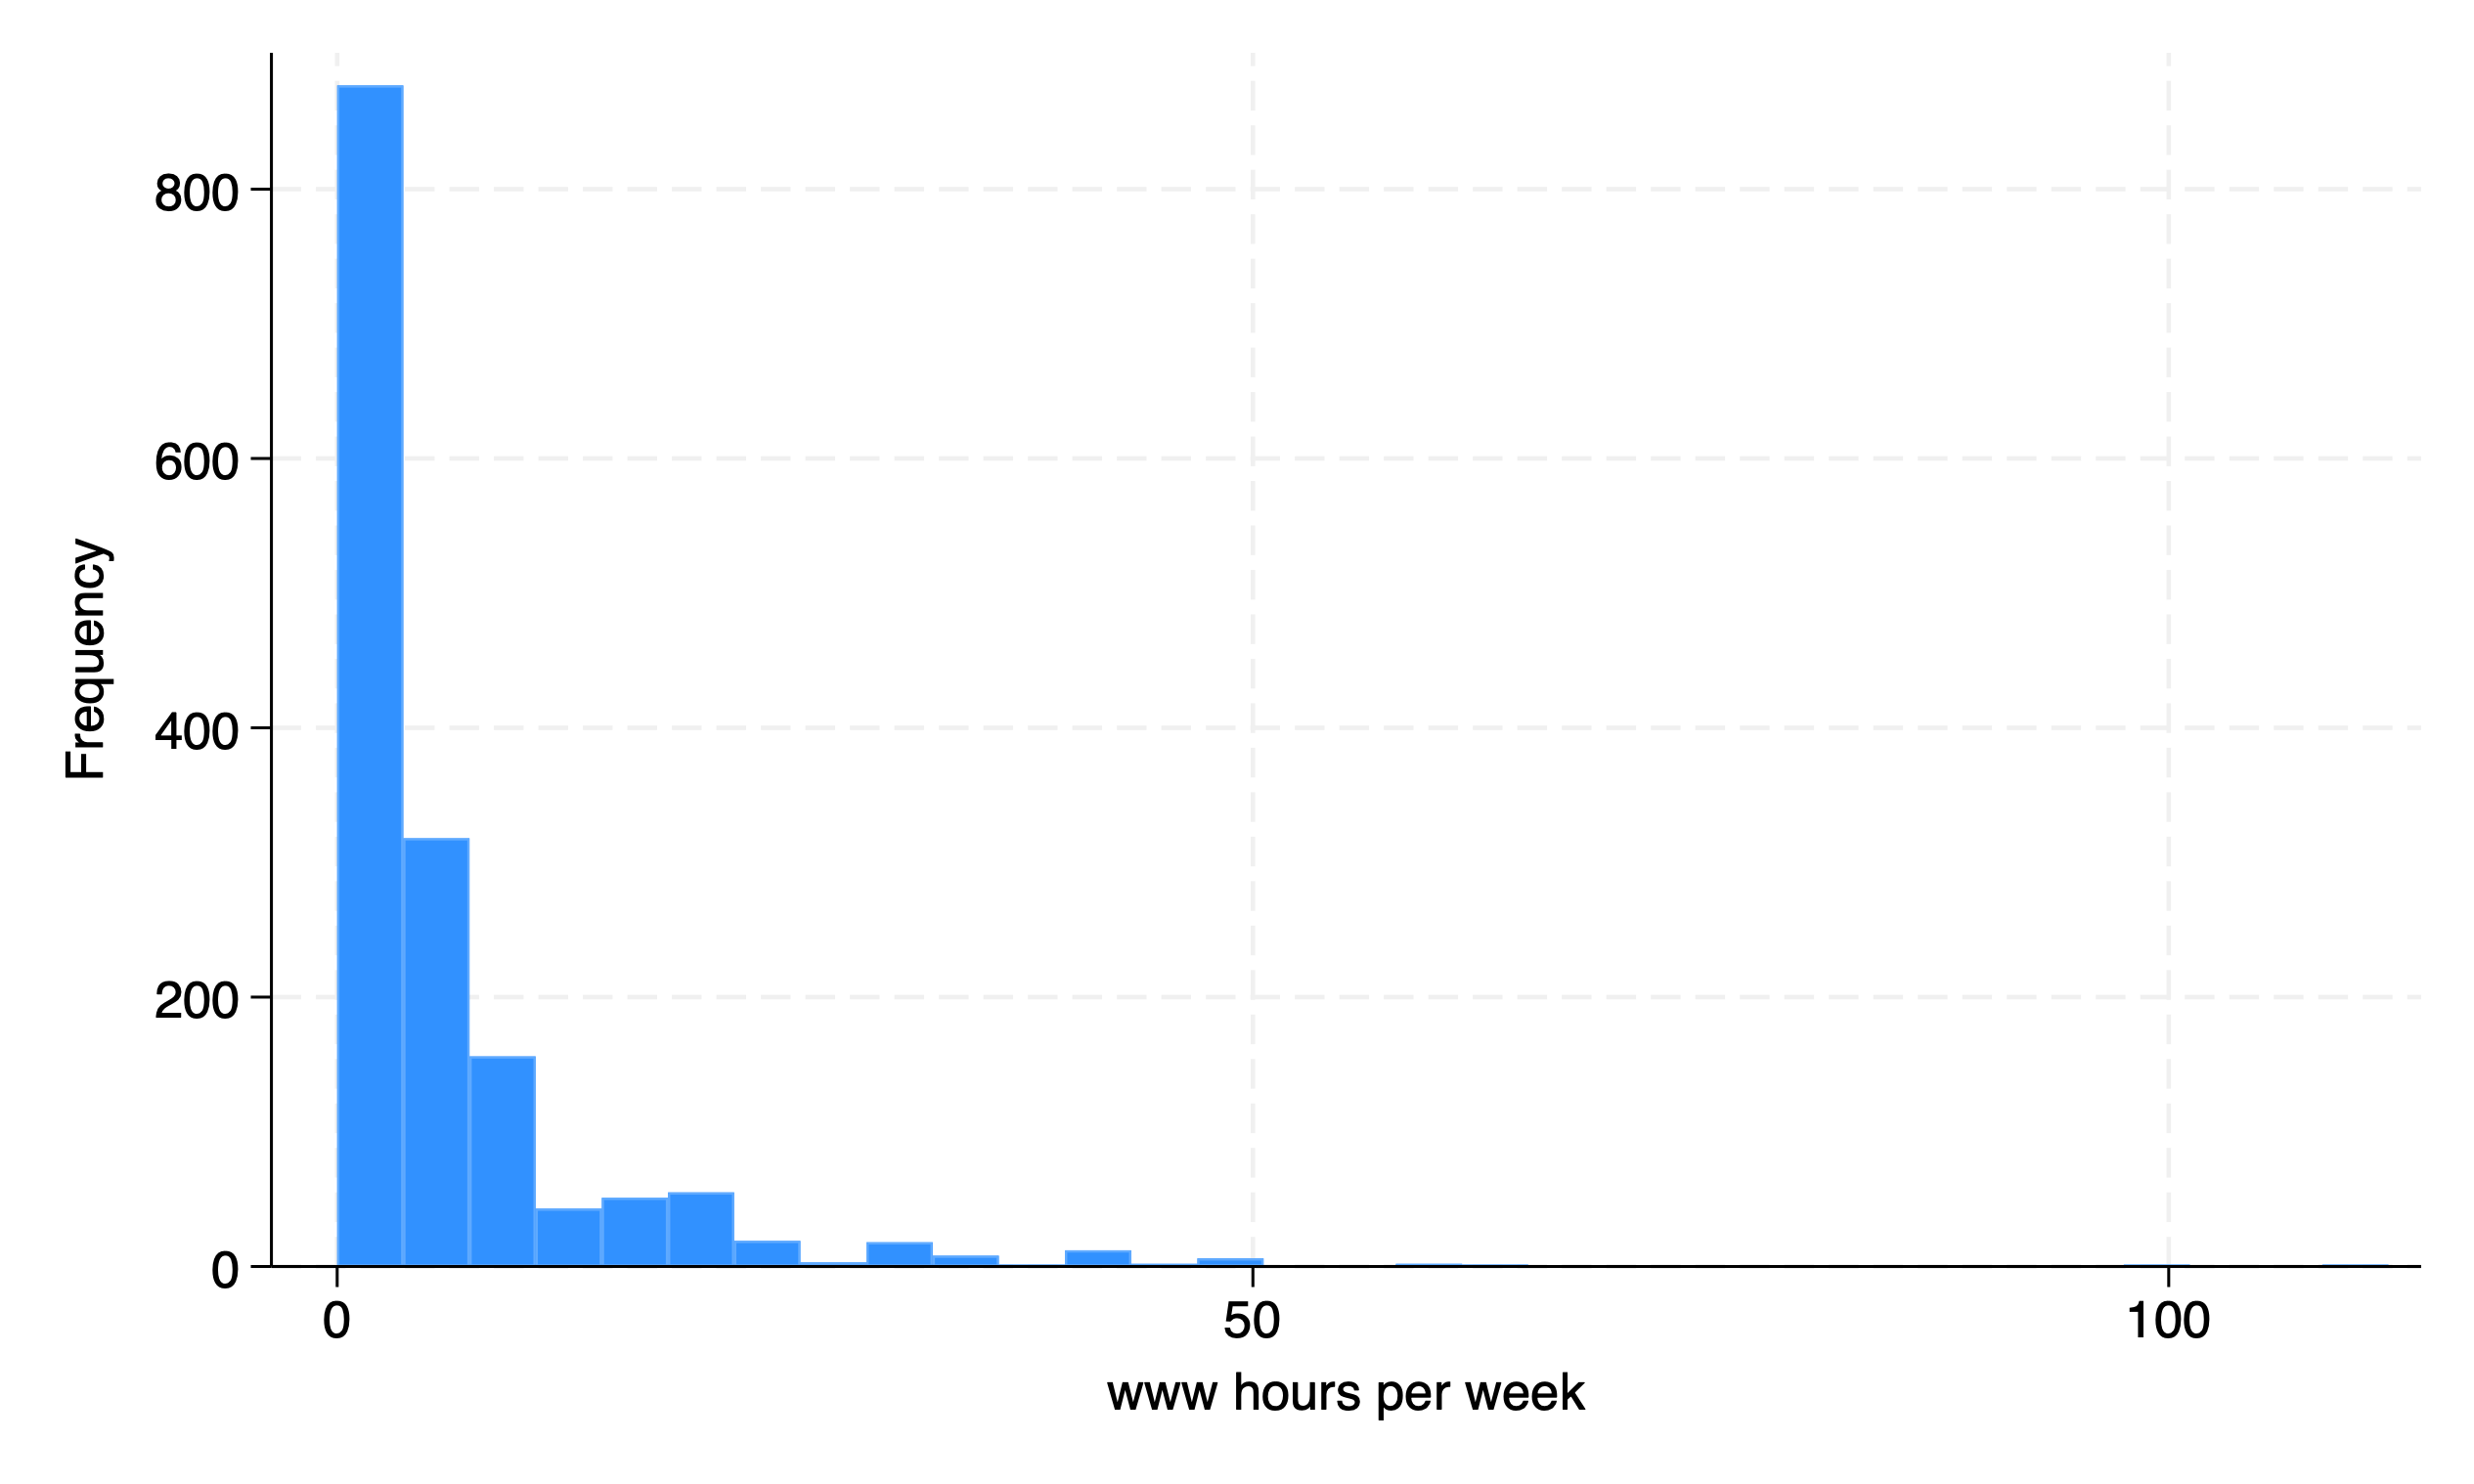
\includegraphics[keepaspectratio,alt={Figure 5.16: Histogram of time spent on the Internet in 2002}]{week3_wwwhr.png}}
\caption{Figure 5.16: Histogram of time spent on the Internet in 2002}
\end{figure}

\begin{Shaded}
\begin{Highlighting}[]
\KeywordTok{histogram}\NormalTok{ hrs1, }\KeywordTok{frequency}
\end{Highlighting}
\end{Shaded}

\begin{figure}
\centering
\pandocbounded{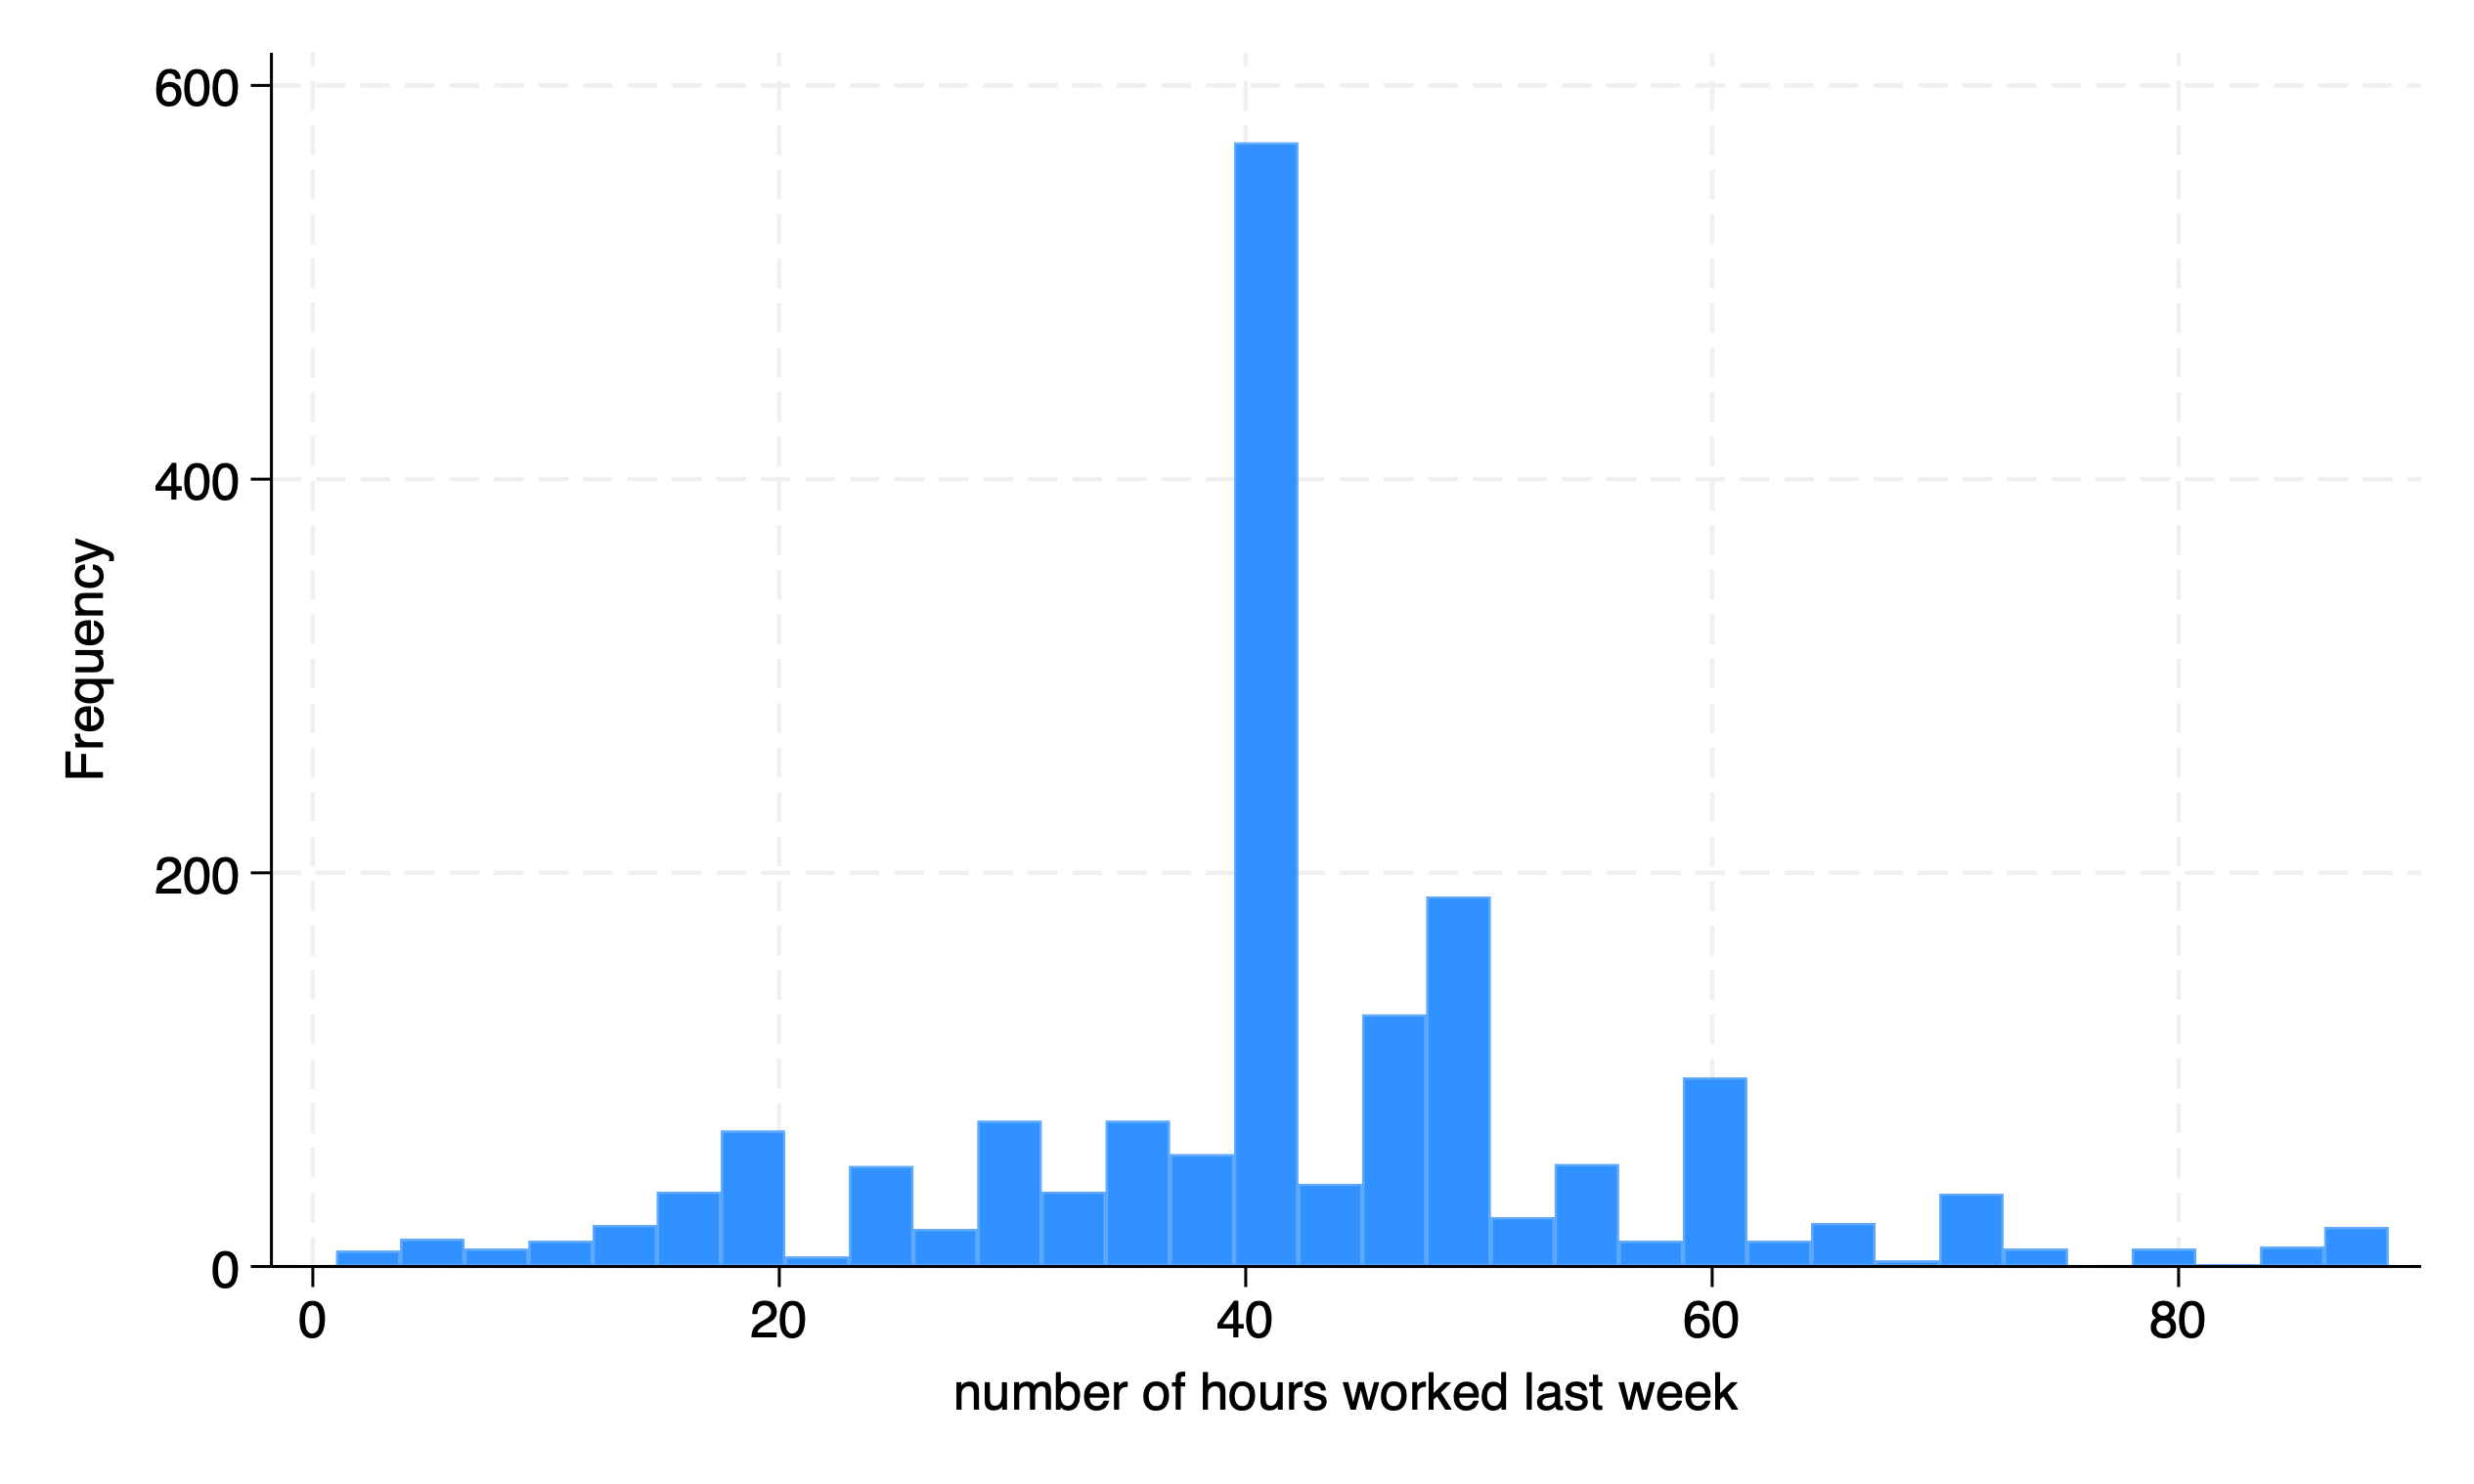
\includegraphics[keepaspectratio,alt={Figure 5.17: Histogram of hours worked per week}]{week3_workhrs.png}}
\caption{Figure 5.17: Histogram of hours worked per week}
\end{figure}

\subsection{Split by another variable}\label{split-by-another-variable}

Next week, we will start to look at two variables, but we can subset our graphs by different groups. Let's look at internet usage in 2002 by women and men. We can use the \emph{by var, sort:} prefix to our command to sort the data by sex.

\begin{Shaded}
\begin{Highlighting}[]
\KeywordTok{by}\NormalTok{ sex, }\KeywordTok{sort}\NormalTok{: }\KeywordTok{summarize}\NormalTok{ wwwhr}
\end{Highlighting}
\end{Shaded}

\begin{verbatim}
-> sex = male

    Variable |        Obs        Mean    Std. dev.       Min        Max
-------------+---------------------------------------------------------
       wwwhr |        711    7.106892     9.98914          0        112

---------------------------------------------------------------------------------------------------------------------
-> sex = female

    Variable |        Obs        Mean    Std. dev.       Min        Max
-------------+---------------------------------------------------------
       wwwhr |        863    4.920046    7.688655          0        100
\end{verbatim}

We can use the \emph{table} command to show descriptive statistics. We can ask fo rthe mean, median, standard deviation, interquartile range, skewness, kurtosis, and coefficient of variation. The \emph{table} command has \emph{rowvars} in the first parathesis and \emph{colvars} in the second parathesis. So we will use sex as the rows and our descriptive statistics in the columns of our table.

\begin{Shaded}
\begin{Highlighting}[]
\KeywordTok{table}\NormalTok{ (sex) (result), statistic(}\KeywordTok{mean}\NormalTok{ wwwhr) statistic(p50 wwwhr) statistic(}\FunctionTok{sd}\NormalTok{ wwwhr) statistic(}\FunctionTok{iqr}\NormalTok{ wwwhr) statistic(skewness wwwhr) statistic(kurtosis wwwhr) statistic(cv wwwhr)}
\end{Highlighting}
\end{Shaded}

\begin{verbatim}
                |      Mean   50th percentile   Standard deviation   Interquartile range   Skewness   Kurtosis   Coefficient of variation
----------------+------------------------------------------------------------------------------------------------------------------------
respondents sex |                                                                                                                        
  male          |  7.106892                 4              9.98914                     9   3.608189    25.2577                   1.405557
  female        |  4.920046                 2             7.688655                     4   4.409274   36.78389                    1.56272
  Total         |  5.907878                 3             8.866734                     6   3.997908   30.39248                   1.500832
-----------------------------------------------------------------------------------------------------------------------------------------
\end{verbatim}

We can export our table as well with the \emph{collect} command after the \emph{table} command. I recommend that you have export functionality in your scripts. This will reduce copy and paste requirements. You can export into a Word document, Excel document, PDF, HTML, \(LaTex\), SMCL, or Markdown.

We will export a Word docx file and a Markdown file.

\begin{Shaded}
\begin{Highlighting}[]
\NormalTok{collect }\KeywordTok{export}\NormalTok{ wwwhr.docx}
\NormalTok{collect }\KeywordTok{export}\NormalTok{ wwwhr.md}
\end{Highlighting}
\end{Shaded}

\begin{figure}
\centering
\pandocbounded{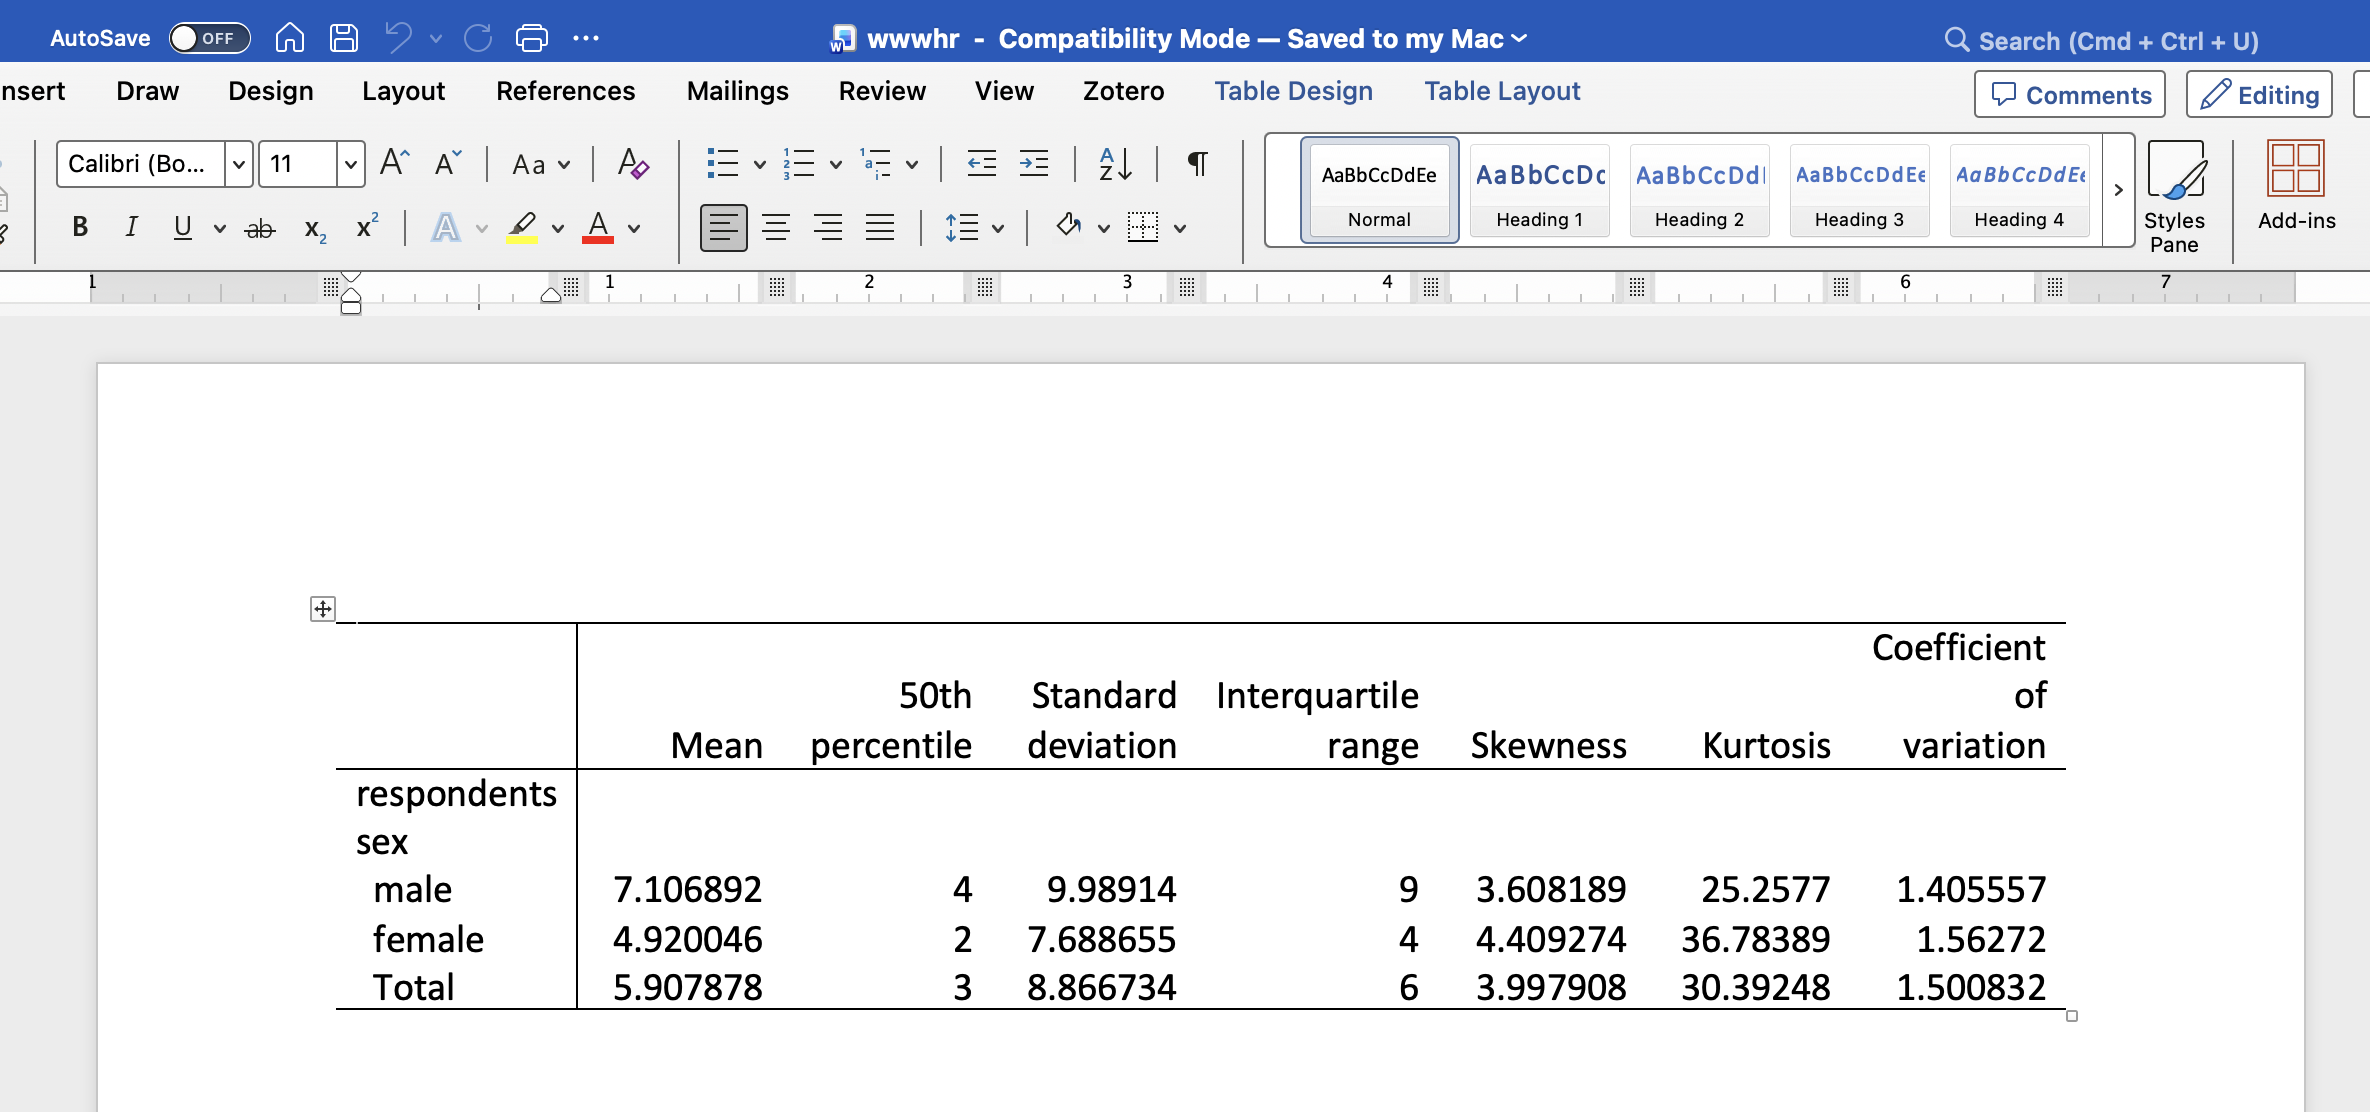
\includegraphics[keepaspectratio,alt={Figure 5.18: Microsoft Word document with results}]{week3_exportdocx.png}}
\caption{Figure 5.18: Microsoft Word document with results}
\end{figure}

\begin{longtable}[]{@{}
  >{\raggedright\arraybackslash}p{(\linewidth - 14\tabcolsep) * \real{0.1298}}
  >{\raggedright\arraybackslash}p{(\linewidth - 14\tabcolsep) * \real{0.0763}}
  >{\raggedright\arraybackslash}p{(\linewidth - 14\tabcolsep) * \real{0.1298}}
  >{\raggedright\arraybackslash}p{(\linewidth - 14\tabcolsep) * \real{0.1527}}
  >{\raggedright\arraybackslash}p{(\linewidth - 14\tabcolsep) * \real{0.1603}}
  >{\raggedright\arraybackslash}p{(\linewidth - 14\tabcolsep) * \real{0.0763}}
  >{\raggedright\arraybackslash}p{(\linewidth - 14\tabcolsep) * \real{0.0763}}
  >{\raggedright\arraybackslash}p{(\linewidth - 14\tabcolsep) * \real{0.1985}}@{}}
\toprule\noalign{}
\begin{minipage}[b]{\linewidth}\raggedright
\end{minipage} & \begin{minipage}[b]{\linewidth}\raggedright
Mean
\end{minipage} & \begin{minipage}[b]{\linewidth}\raggedright
50th percentile
\end{minipage} & \begin{minipage}[b]{\linewidth}\raggedright
Standard deviation
\end{minipage} & \begin{minipage}[b]{\linewidth}\raggedright
Interquartile range
\end{minipage} & \begin{minipage}[b]{\linewidth}\raggedright
Skewness
\end{minipage} & \begin{minipage}[b]{\linewidth}\raggedright
Kurtosis
\end{minipage} & \begin{minipage}[b]{\linewidth}\raggedright
Coefficient of variation
\end{minipage} \\
\midrule\noalign{}
\endhead
\bottomrule\noalign{}
\endlastfoot
respondents sex & & & & & & & \\
male & 7.106892 & 4 & 9.98914 & 9 & 3.608189 & 25.2577 & 1.405557 \\
female & 4.920046 & 2 & 7.688655 & 4 & 4.409274 & 36.78389 & 1.56272 \\
Total & 5.907878 & 3 & 8.866734 & 6 & 3.997908 & 30.39248 & 1.500832 \\
\end{longtable}

We can also split the histogram by another variable to see if the distribution varies by sex. We can use the \emph{by(var)} option to accomplish this split. We can also subset hours to less than 25 hours with the qualifier \emph{if wwwhr \textless{} 25}.

\begin{Shaded}
\begin{Highlighting}[]
\KeywordTok{histogram}\NormalTok{ wwwhr }\KeywordTok{if}\NormalTok{ wwwhr \textless{} 25, }\KeywordTok{frequency} \KeywordTok{by}\NormalTok{(sex)}
\end{Highlighting}
\end{Shaded}

\begin{figure}
\centering
\pandocbounded{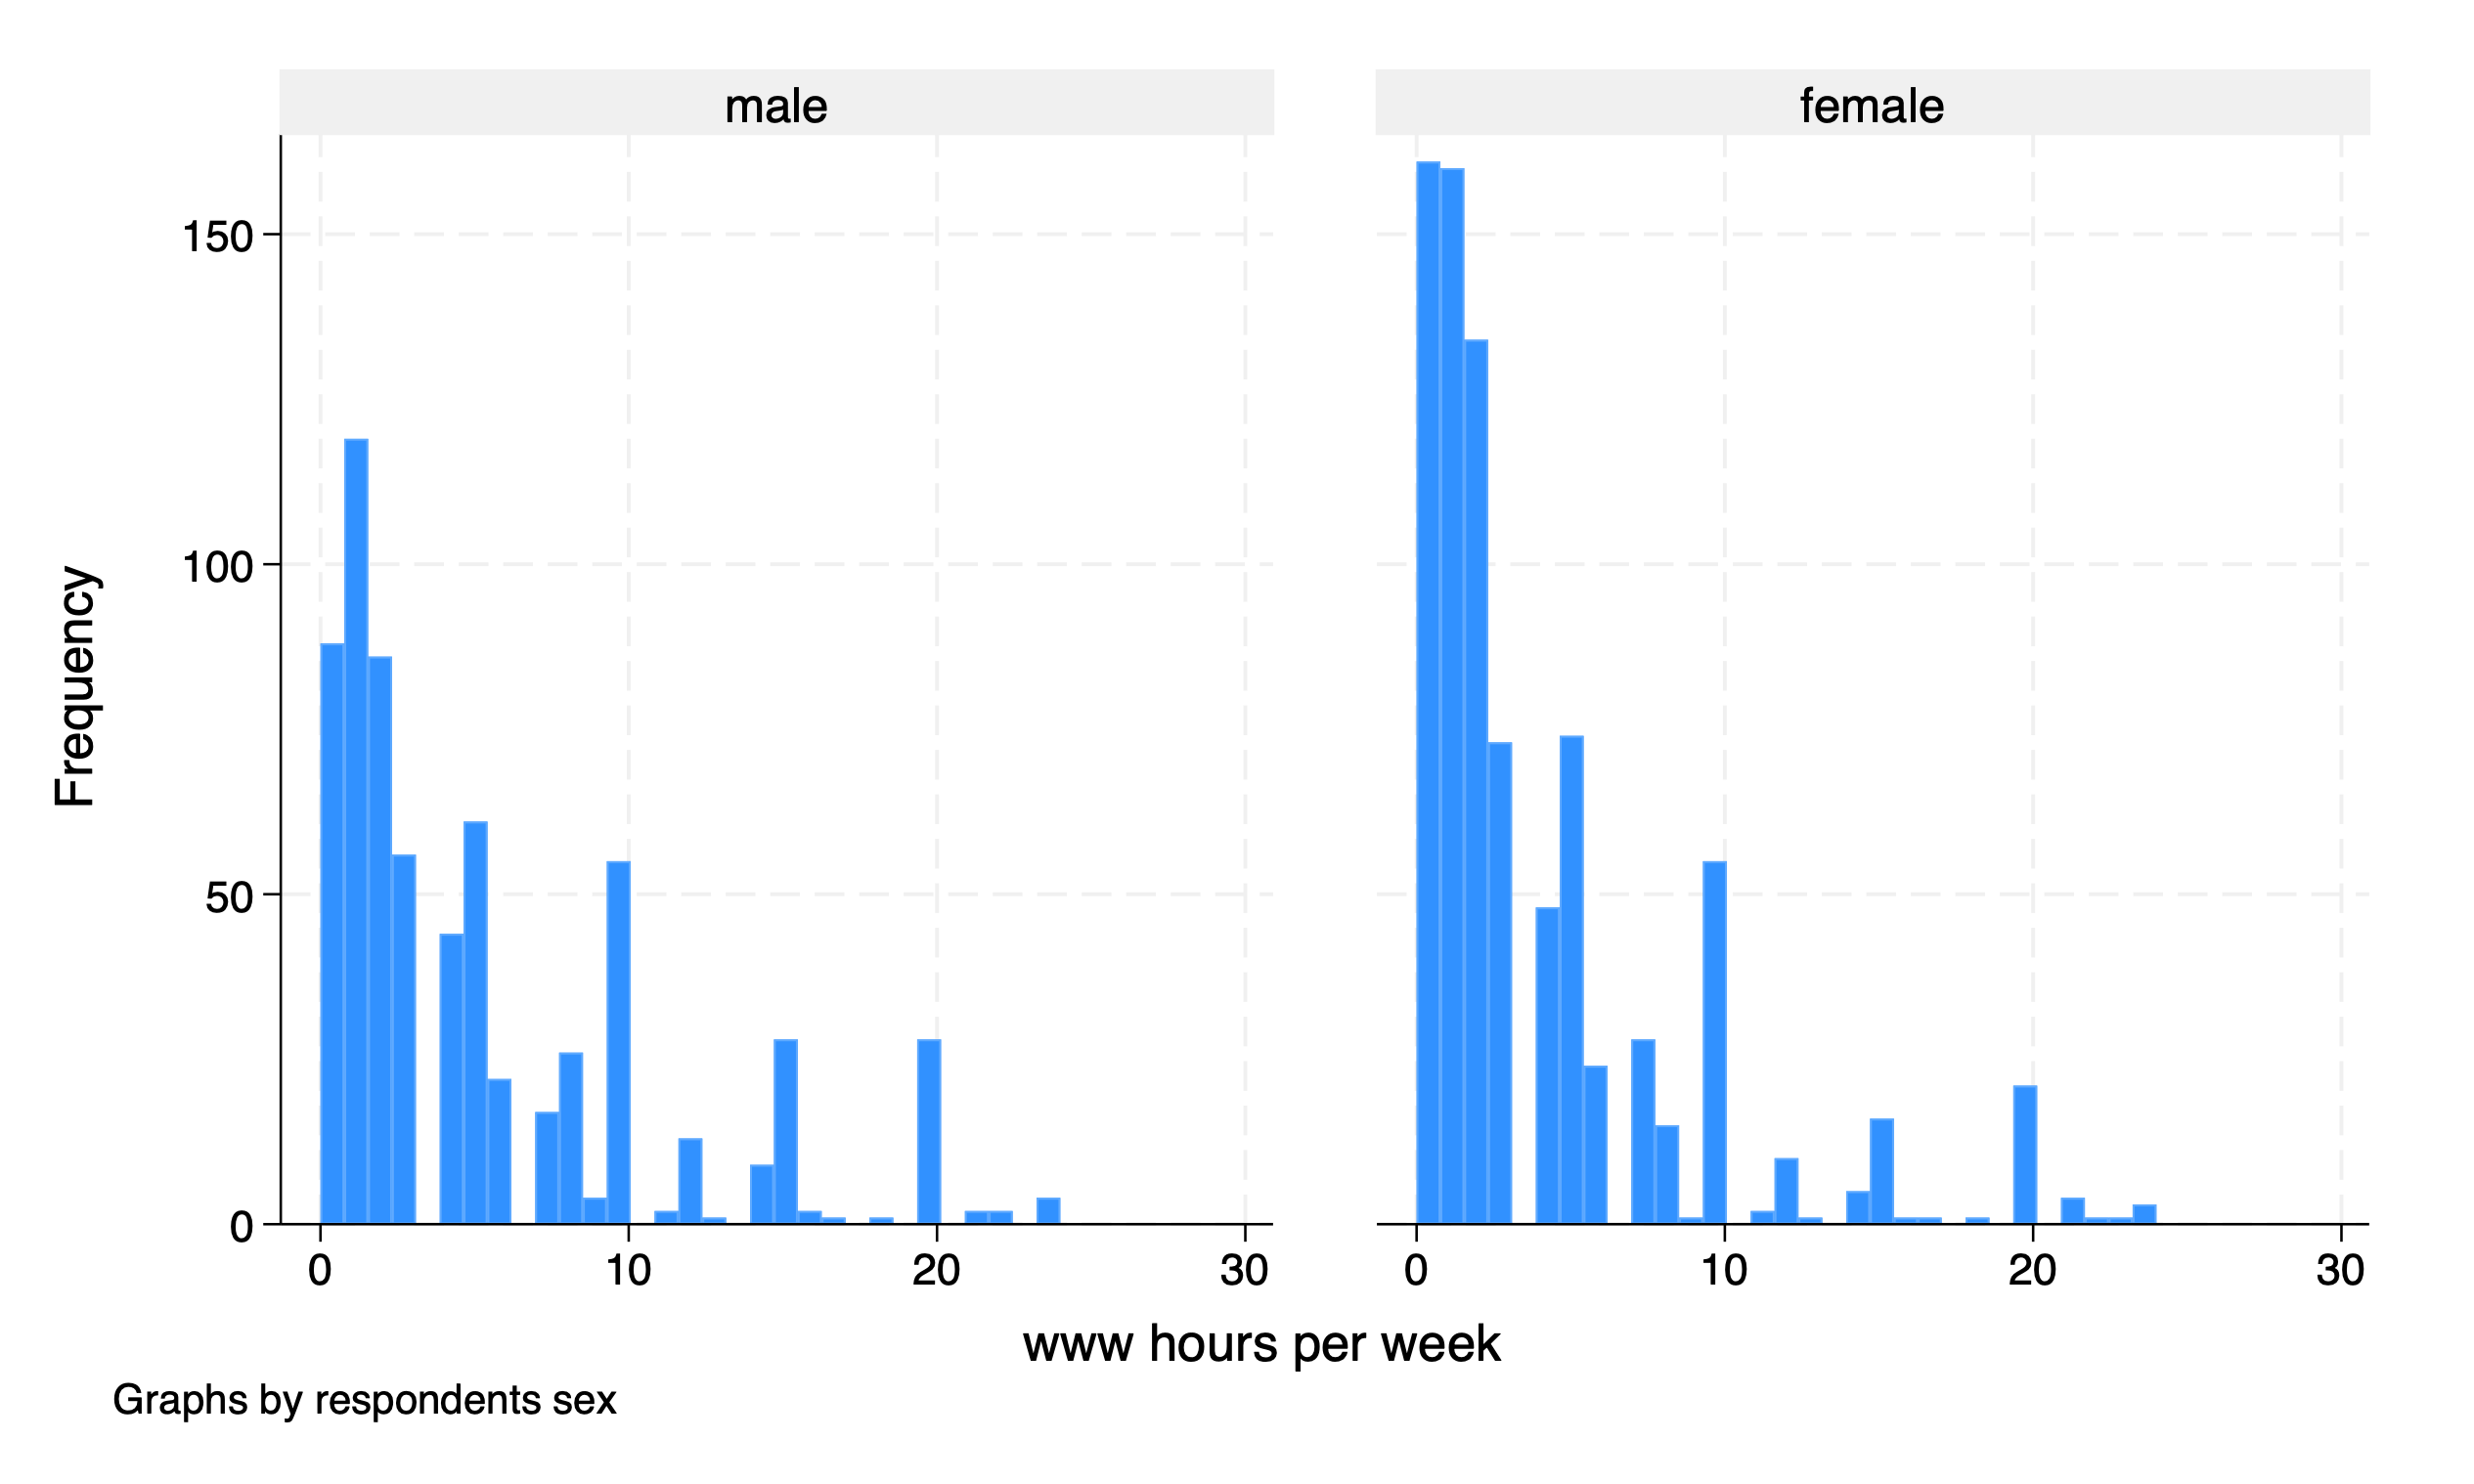
\includegraphics[keepaspectratio,alt={Figure 5.19: Histogram of time spent on the Internet in 2002 by sex for under 25 hours per week}]{week3_histbysex.png}}
\caption{Figure 5.19: Histogram of time spent on the Internet in 2002 by sex for under 25 hours per week}
\end{figure}

\subsection{Box Plots}\label{box-plots}

Our file set of graphs is the box plot. We can calculate and graph box plots with the command \emph{graph hbox} command for horizontal box plots. We will add the option \emph{over(sex)} to split the data into women and men.

\begin{Shaded}
\begin{Highlighting}[]
\KeywordTok{graph}\NormalTok{ hbox wwwhr }\KeywordTok{if}\NormalTok{ wwwhr \textless{} 25, }\BaseNTok{over}\NormalTok{(sex) }\BaseNTok{title}\NormalTok{(}\StringTok{"Hours spent on the Internet"}\NormalTok{) }\BaseNTok{subtitle}\NormalTok{(}\StringTok{"By sex"}\NormalTok{) }\BaseNTok{caption}\NormalTok{(}\StringTok{"descriptive\_gss.dta"}\NormalTok{) }\DecValTok{scheme}\NormalTok{(economist)}
\end{Highlighting}
\end{Shaded}

\begin{figure}
\centering
\pandocbounded{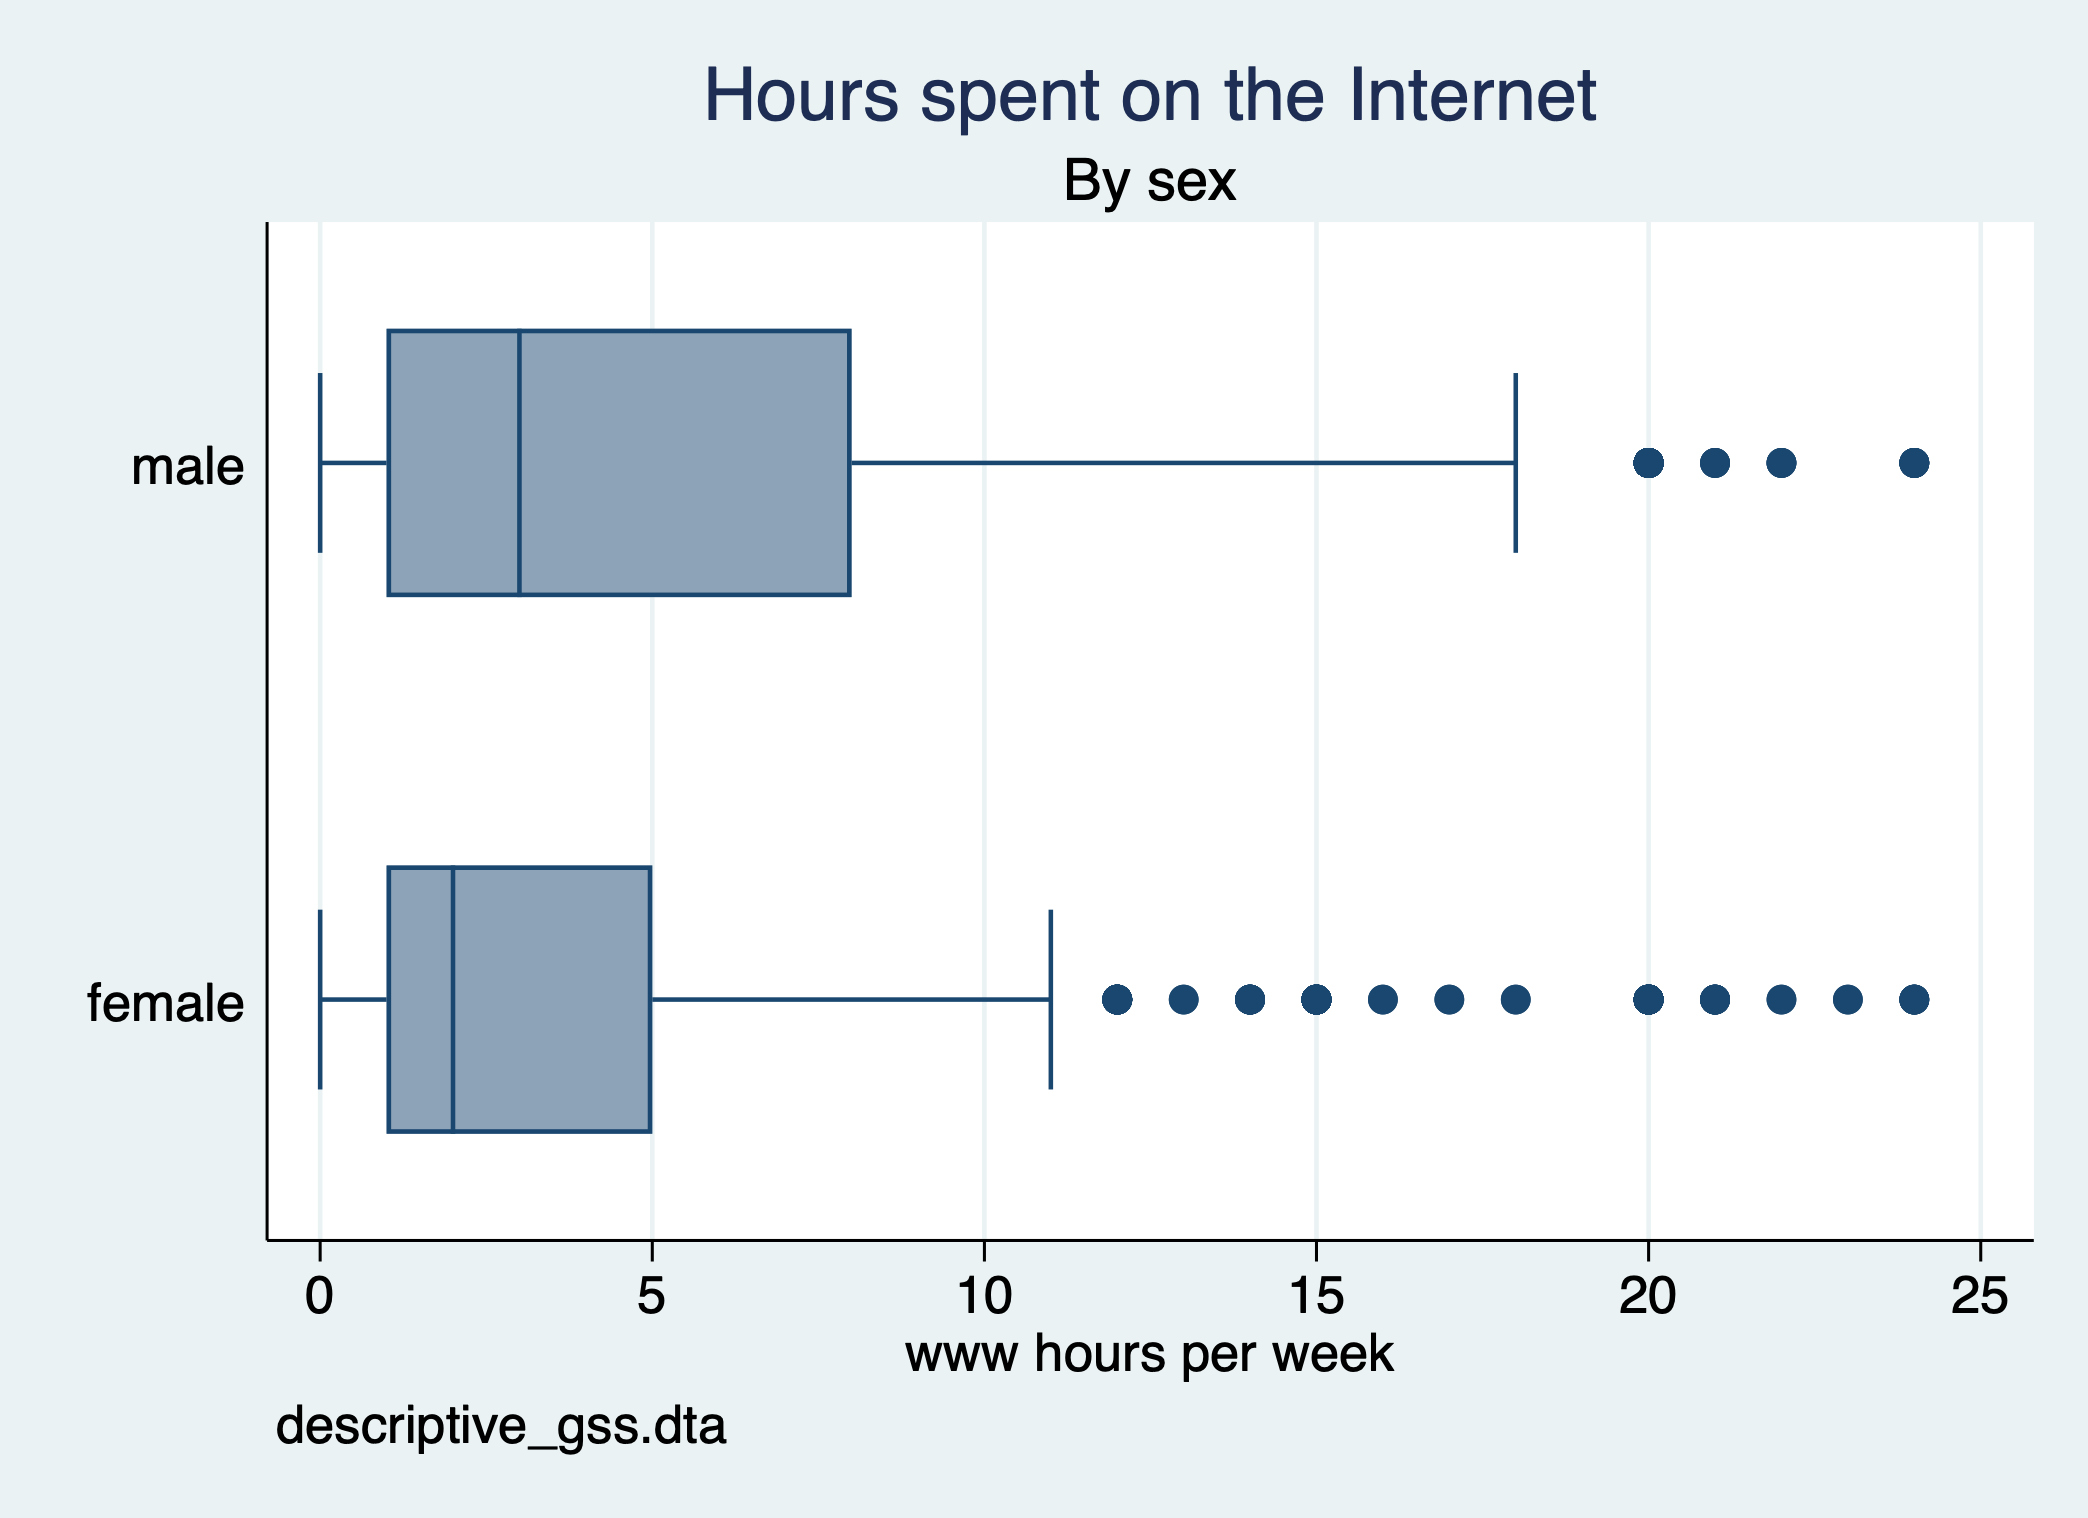
\includegraphics[keepaspectratio,alt={Figure 5.20: Box plot of time sepnt on the Internet for less than 25 hours per week by sex}]{week3_boxplot.png}}
\caption{Figure 5.20: Box plot of time sepnt on the Internet for less than 25 hours per week by sex}
\end{figure}

\chapter{Exercises}\label{exercises}

We will practice calculating and displaying descriptive statistics for one variable. Please complete the following exercises.

\section{General Social Survey}\label{general-social-survey}

We will use ``descriptive\_gss.dta'' from Acock (2023). Ingest the data into Stata to complete the exercises.

\subsection{Nomimal Variables}\label{nomimal-variables}

Steps

\begin{enumerate}
\def\labelenumi{\arabic{enumi}.}
\tightlist
\item
  Compute a frequency tabulation of marital status
\item
  What is the mode of marital status?
\end{enumerate}

\subsection{Ordinal Variables}\label{ordinal-variables}

Steps

\begin{enumerate}
\def\labelenumi{\arabic{enumi}.}
\tightlist
\item
  Compute a frequency tabulation of \emph{strsswkr}.
\item
  What is the mode? What does it mean?
\item
  Calculate the median. Is it the same as the mode?
\item
  Display a histogram of the variable using the \emph{discrete} and \emph{frequency} options.
\item
  Display a bar chart of the variable using \emph{(count), over(strsswrk)}
\end{enumerate}

\subsection{Quantitative Variables}\label{quantitative-variables-1}

Steps

\begin{enumerate}
\def\labelenumi{\arabic{enumi}.}
\tightlist
\item
  Use a tabulation for the discrete variable \emph{educ}
\item
  What is the mode for years of education?
\item
  Calculate the mean and median of \emph{educ}
\item
  Are the median and mean the same as the mode?
\item
  Display a bar graph of \emph{educ}
\item
  Question: is this a discrete variable or can it be an ordinal variable?
\end{enumerate}

Steps

\begin{enumerate}
\def\labelenumi{\arabic{enumi}.}
\tightlist
\item
  Calculate the mean and median of \emph{age}
\item
  Is the mean and median equal to zero or do they differ?
\item
  Is the skewness near zero?
\item
  What about the kurtosis? Does it tell us anything about the shape of the distribution?
\item
  Display a histogram of \emph{age}
\item
  Does the histogram corroborate the results from \emph{sum}?
\item
  Display a box plot of \emph{age} by sex.
\item
  Do you see any outliers?
\end{enumerate}

\section{Current Population Survey}\label{current-population-survey}

We will use the July 2026 Current Population Survey to use descriptive statistics on wages.

Ingestion Steps

\begin{enumerate}
\def\labelenumi{\arabic{enumi}.}
\tightlist
\item
  Go to the Census Bureau's website and ingest the July 2026 csv file
\item
  \url{https://www2.census.gov/programs-surveys/cps/datasets/2026/basic/jul26pub.csv}
\item
  The data dictionary can be found here: \url{https://www2.census.gov/programs-surveys/cps/datasets/2026/basic/2026_Basic_CPS_Public_Use_Record_Layout_plus_IO_Code_list.txt}
\end{enumerate}

\subsection{Quantitative Variables}\label{quantitative-variables-2}

Descriptive Statistics Steps

\begin{enumerate}
\def\labelenumi{\arabic{enumi}.}
\tightlist
\item
  Our variable of interest is \emph{pternwa}.
\item
  We use a qualifier \emph{prerelg} as a flag for available earnings (prerelg==1)
\item
  Calculate the mean and median of weekly earnings
\item
  There appear to be issues. What do you see?
\item
  Use the command ``gen earnings=pternwa/100''
\item
  Recalculate the mean and median.
\end{enumerate}

Displaying Steps

\begin{enumerate}
\def\labelenumi{\arabic{enumi}.}
\tightlist
\item
  Next, we want to display the distribution of the weekly earnings
\item
  Use a histogram to display the weekly earnings
\item
  Are the data distributed normally?
\item
  Do you notice anything unusual about the distrubtion?
\item
  Next use a box plot to display the distribution of the data.
\end{enumerate}

Acock, A.C. (2023). A gental introduction to stata

\bibliography{book.bib,packages.bib}

\end{document}
